% !Mode:: "TeX:UTF-8"
\documentclass[10pt,journal]{IEEEtran}
\usepackage{subfig}
\usepackage{graphicx}
\usepackage{amsmath}
\usepackage{algorithm}
\usepackage{algorithmic}
\usepackage{comment}
\usepackage{multirow}
\usepackage{diagbox}

\graphicspath{figures/}

\newtheorem{theorem}{Theorem}
\newtheorem{lemma}{Lemma}
\newtheorem{definition}{Definition}

\begin{document}
\title{Delay Analysis and Buffer Optimization for Priority-Aware Networks-on-Chip (NoC)}
%\onecolumn
%\author{\IEEEauthorblockN{Baoliang Li}}

\author{Baoliang~Li, %~\IEEEmembership{Student Member,~IEEE,}
        Zeljko Zilic, %~\IEEEmembership{Senior Member,~IEEE,}
        Wenhua~Dou, %~\IEEEmembership{Non-Member,~IEEE}% <-this % stops a space
\thanks{Baoliang~Li and Wenhua Dou are with the College of Computer Science, National University of Defense Technology, Changsha 410073, P.R. China}%
\thanks{Zeljko Zilic are with Department of Electrical \& Computer Engineering, McGill University, Montreal H3A-2A7, Quebec, Canada}%
\thanks{Manuscript received XX XX, 2014; revised XX XX, 2014.}}

\markboth{Journal of XXX,~Vol.~XX, No.~XX, XX~2014}%
{Li \MakeLowercase{\textit{et al.}}: A Delay and Backlog Model for Priority-Aware Networks-on-Chip (NoC)}

\maketitle

\begin{abstract}
Among all the implementation alternatives of Networks-on-Chip (NoC), priority-aware wormhole-switched NoC is promising to meet both the worst-case and average-case latency requirements of on-chip communication. The worst-case end-to-end latency and buffer requirement analysis are very important for the development of real-time applications on this platform, Link-Level Analysis (LLA) and Deterministic Network Calculus (DNC) have been successfully applied to achieve this goal. In this paper, we first propose a Real-Time Calculus (RTC) based performance model for the priority-aware NoC. Then, we propose an end-to-end latency analysis algorithm and a buffer optimization algorithm. The latency analysis algorithm can give much tighter delay bound than DNC, since it take the maximum service capacity and minimum arrival traffic into consideration. The buffer optimization algorithm try to reduce the buffer space required for each flow without violating the deadline, which improves the existing backlog bound obtained by LLA. Our algorithms are topology-independent, it takes as input the network topology graph and the application traffic characterization, and gives the end-to-end latency and buffer requirement for each traffic flow. Our model enables the fast performance evaluation and buffer optimization of priority-aware NoC, which can be used for application mapping, routing selection and power reduction. Experiment results demonstrate the effectiveness and tightness of our model. In addition, further comparisons with other theoretical models also indicates that, our method outperforms the existing methods while the tightness of the derived delay and backlog bound are considered.
\end{abstract}
\begin{IEEEkeywords}
Networks-on-Chip (NoC), priority-aware, real-time calculus, delay bound, buffer optimization
\end{IEEEkeywords}

\section{Introduction}
The conventional on-chip interconnection paradigms, e.g. bus, ring and point-to-point links, are not able to meet the strict and complex communication requirements of modern large scale Chip-MultiProcessors (CMPs) and System-on-Chip (SoC). As an alternative, Networks-on-Chip (NoC) is proposed to provide better scalability, higher power efficiency, and low-latency global communication. As a key component of CMPs and SoC, NoC must be well designed to meet the rigorous requirements on end-to-end latency, buffer constraint, throughput and power, etc. Although various proposals have been emerged, with each focusing on improving different performance metrics of on-chip communication, most of the existing research on NoC are focusing on the improvement of average performance of on-chip wormhole-switched network, and simulation is the widely used performance evaluation method. Whereas, there also exists lots of on-chip applications, which are sensitive to the worst-case or real-time communication performance of NoC, e.g. cache coherent protocol \cite{Bolotin2007} and multimedia application \cite{ostermann2004video}. How to design the on-chip communication infrastructure for these applications and analyze its feasibility are of big challenges for the researchers.

To meet the rigorous Quality-of-Service (QoS) requirement, various special hardware implementations have been proposed, e.g. Time-Division Multiplexing-Access (TDMA) \cite{GoDR05}, circuit-switch \cite{6628254} and time-triggered switch \cite{4617280}. Although provide strict real-time communication guarantee, the average performance and resource utilization of these proposals are very poor. In contrast, wormhole-switched NoC is widely used in on-chip network due to its simplicity and high-efficiency. Thus, providing real-time communication support on the conventional wormhole-switched NoC to meet both average-case and worst-case communication requirements is the most promising solution. To achieve this goal, a special scheduling policy (e.g. DifServ \cite{1411140} or priority-aware implementation \cite{Shi:2008:RCA:1397757.1397996}\cite{708526}\cite{627905}) or flow control mechanism (e.g. \cite{Li199649}\cite{707545}) should be implemented. For all these wormhole-switch based real-time communication proposals, a key step before their adoption as a platform of real-time applications is the analysis of the worst-case communication latency for all the real-time flows to guarantee the satisfaction of deadline constraint. In addition, an effective buffer analysis approach is also needed to optimize the buffer allocation under real-time constraint, since the buffer usually consumes about 46\% power \cite{pkundu} and occupies 30\% area \cite{5507566} of entire router.

A creditable and accurate worst-case analysis is crucial for the application of wormhole-switched NoC in real-time communication, since an over optimistic estimation will lead to the violation of deadline, while an over pessimistic estimation will make the utilization of on-chip resource very low. The conventional simulation based method might not be competent for the worst-case analysis, this is because the worst-case scenarios are hard to be captured by simulation. As an alternative, the analytical method can establish the relationship between performance metrics and design parameters in a very short time, and give the worst-case performance immediately. For the worst-case analysis of fixed-priority wormhole-switched on-chip networks, Flow-Level Analysis (FLA) \cite{Shi:2008:RCA:1397757.1397996}, Link-Level Analysis (LLA) \cite{73}\cite{189} and Deterministic Network Calculus (DNC) \cite{Qian489900} have been successfully applied. Both FLA and LLA have their roots in the classic scheduling theory, which assume that, the traffic flows are strictly periodic, and the input buffer of wormhole-switched NoC is sufficient large, so that the back-pressure caused by flow control can be ignored. In addition, they simplified the router model by restricting the per-hop latency to be one cycle, which is complying with the conventional router implementation.

Deterministic network calculus overcomes these limitations by applying the advanced operators in dioid algebra. However, we found that the DNC based latency bound can be further improved, because the DNC based method \cite{Qian489900} ignored the maximal service capacity of on-chip routers, which has significant impact on the tightness of output arrival curve served by a specific router. The over estimated output arrival curve in \cite{Qian489900} will further lead to a looser leftover service curve and looser performance bounds for the low-priority flows. To overcome this shortcoming of DNC, we adopt the real-time calculus (RTC) theory \cite{1253607} originally used for the real-time task scheduling analysis to build an end-to-end performance model for the wormhole-switched NoC with credit-based flow control. Compared with DNC model in \cite{Qian489900}, the RTC model in this paper utilize the maximal service curve and minimal arrival curve to limit the output arrival curve and left service curve, which significantly improve the tightness of performance bound. We will further explain the reason and demonstrate the improvement in Section \ref{experiments}.

The main contribution of this paper is two folded: (1) We propose an end-to-end latency analysis algorithm for the priority-aware NoC based on the RTC model, compared with the existing DNC \cite{Qian489900} method, it can give a tighter performance bound. The output of this algorithm can be used as the reference of IP core mapping, task mapping, routing selection, or NoC parameters configuration; (2) We also propose an RTC based buffer optimization algorithm for the application-specific NoC to reduce the buffer size under deadline constraint. This is an significant improvement of previously proposed FLA and LLA based buffer optimization method \cite{189}, because the previous methods can only be applied to compute the minimal buffer-size that does not trigger the flow control. This algorithm can be used to minimize the power consumption and chip area.

The rest of this paper is organized as follows: we present the existing real-time communication proposals and its related performance analysis methods in Section \ref{related}. In Section \ref{model}, the basic assumptions on wormhole switched NoC and a brief introduction to RTC theory is presented. The detailed modeling process is presented in Section \ref{modeling}, where we also propose an end-to-end latency analysis algorithm and a buffer optimization algorithm. We present the experiment results and comparison with other analytical methods in Section \ref{experiments}. Finally, we summarize our paper in Section \ref{conclusion}.

\section{Related Work}\label{related}
Since first introduced in 2001 \cite{DaTo01}, various NoC proposals have been emerged to meet different on-chip communication requirements. The main requirements posed to NoC by on-chip applications are latency and bandwidth. To meet these demand, NoC are designed to be either best-effort or guaranteed-service, depending on the hardware cost and application requirement. The performance evaluation of these two categories include the average analysis and worst-case analysis. For the average analysis, simulation and probability-based approach hold the dominant position for both best-effort and guaranteed-service NoC. However, for the worst-case analysis, simulation is not competent due to the difficulty in covering all the corner cases. The analytical worst case analysis for these two categories is also slightly different. Synchronous Data Flow (SDF) graph \cite{poplavko2003task} and DNC \cite{qian2009analysis} have been presented to model the worst case performance bound of best-effort NoC. The former method assumes the traffic flow to be periodical, and the latter one eliminates this constraint to allow the traffic to be arbitrary patterns. In \cite{qian2009analysis}, the authors build an analytical performance model with DNC taking the various contention and flow control into consideration. This result is further extended in \cite{Du:2012:WPA:2380445.2380469}, where the traffic splitter was proposed to support the multi-path routing polices. Another method is presented in \cite{Lee:2003:RWC:846077.846083} to compute the worst-case latency for conventional wormhole switched network, and a real-time Wormhole Channel Feasibility Checking (WCFC) algorithm is proposed. This research is further extended to calculate the bandwidth and latency bound in \cite{6109240}, and used for topology synthesis of best-effort NoC in \cite{EPFL-ARTICLE-186879}.

A simple and effective solution to provide guaranteed-service for different applications is classifying these applications into several service classes, each with different priorities, and the network provides services according to the priority of each class. Representative implementations of this idea include QNoC \cite{BCGK04}, fixed-priority NoC \cite{Shi:2008:RCA:1397757.1397996} and {{\AE}thereal} \cite{GoDR05} etc. In \cite{LuJS05}, contention tree model was proposed to analyze the feasibility of real-time traffic delivered by priority-aware wormhole-switched NoC. It improves the previous results, e.g. lumped link model \cite{707545} and dependency graph model \cite{708526}, by allowing the concurrent link usage. This is similar as the the LLA \cite{73}, which improves the FLA proposed in \cite{Shi:2008:RCA:1397757.1397996} by treating each link segment separately. A comprehensive comparison between FLA, contention tree model \cite{LuJS05}, lumped link model \cite{707545} and dependency graph model \cite{708526} can be found in \cite{Shi2009}, in which several defects of previous works are illustrated. Two buffer sizing method based on FLA and LLA, i.e. Flow-Level Buffer-space Analysis (FLBA) and Link-Level Buffer-space Analysis (LLBA), are proposed in \cite{189} to estimate the buffer size of priority-aware wormhole-switched NoC. The main drawback of FLA and LLA is that, these methods require the traffic arrive periodically and the router has single cycle latency, which are significant simplification to the realistic traffic pattern and router implementation. In addition, the FLBA and LLBA can only compute the minimum backlog bound at each router which does not trigger the flow control. In fact, we can further reduce the buffer size as long as the the flow control does not cause the violation of deadline.

On the other hand, although the DNC based analytical method in  \cite{qian2009analysis} can be applied to the analysis of priority-aware NoC, the obtained performance bound is very conservative, especially for the high priority flows. This is because, it does not take the priority-aware scheduling into consideration. To overcome this limitation, an DNC model is proposed to analyze the worst case latency of priority-aware NoC \cite{Qian489900}. But we found that, the DNC method in \cite{Qian489900} can be further improved if we take the maximum service curve of each router and minimum arrival curve of each flow into consideration, this is because the maximal service curve and minimum arrival curve can limit the output arrival curve and improve the leftover service curve for low-priority flows (please refer to Theorem 1.6.2 in \cite{Boudec2001Network} for the reason). Motivated by this observation, we adopt the RTC theory \cite{1253607} to compute the worst-case end-to-end performance of priority-aware wormhole-switched NoC. Real-time calculus is the extension of DNC theory by integrating the maximum service curve and lower arrival curve, which has been widely used in the modeling and analysis of network processor \cite{1253838}, CAN \cite{4617308}, FlexRay \cite{Hagiescu:2007:PAF:1278480.1278554} and DSP systems \cite{thiele2005performance}, etc. To ease the application of RTC, a real-time calculus toolbox \cite{rtc} has also been implemented to support the numerical calculation.

\section{Preliminaries}\label{model}
\subsection{Basic Assumptions}
For the detailed description of generic NoC architecture, please refer to \cite{jerger2009chip}. In this paper, we consider the same network model as in \cite{627905}\cite{Shi:2008:RCA:1397757.1397996}\cite{707545}\cite{73}: Each router has the same number of input and output port, and each input port has sufficient FIFO buffers, i.e. Virtual Channel (VC), to accommodate all the incoming traffic of different priority level. The allocation of VC is determined by the VC allocator. To ensure the predicable transmission of message, we assume that, a deterministic routine computation module is used to determine the output port of each communication message. Crossbar is used to switch traffic from input ports to the output ports, and the switch operation is determined by the switch allocator. We assume the switch allocator is priority-aware: if multiple flits from different input ports or different VCs of the same input port contend for the same output port, it will only grant the flit with highest priority. Flits from a lower priority can transmit a flit if and only if there are no flits from higher priority in the input buffer or the flits with higher priority are self-blocked due to the insufficiency of VC buffer at downstream router. In addition, we also assume that, the buffer depth of each VC is finite, and credit-based flow control is adopted between each router.

The router micro-architecture considered here has 5 pipeline stages, i.e. Buffer-Write (BW), Route Computation (RC), VC Allocation (VA), Switch Allocation (SA), Switch Traversal (ST) and Link Traversal (LT). Although we focus on the standard 5-stage router, our method can be easily modified to support the speculation-based router, e.g. routers with only 2 or 3 stages, the only difference is the initial delay of our model. Communication message is broken input packets, and each packet is composed of one head flit, one tail flit and several body flits. Each head flit should traverse all the five stages to find a path and reserve VC for the follow non-head flits. Non-head flits skip the RC and VA stage since the routine and VC have been determined by head flit. Router resource and control information reserved for a packet will be released only after the tail flit of this packet has been departed from the router. An additional priority field in the head flit is required for the routers to scheduling multiple contending flows according to their priority. To simplify of our analysis, we also assume that, the entire chip use synchronous design, the frequency and period of clock are $f$ and $T$, respectively. Our method can also be applied to analyze Global Asynchronous Local Synchronous (GALS) NoC with little modification, because the routers located in different voltage-frequency islands can be synchronized with a half cycle synchronizer \cite{5476986}, corresponding to a fixed-latency element in DNC theory.

Our performance model is topology independent, but to demonstrate the basic idea of our method, we take the mesh topology as an example, as shown in Fig. \ref{topology}. The router in mesh topology has five ports, corresponding to the four cardinal directions (West, East, North and South) and the Network Interface (NI), which connects to the local Intellectual Property (IP) core. There are 4 traffic flows in Fig. \ref{topology}, i.e. $f_1$, $f_2$, $f_3$ and $f_4$. A flow is a sequence of packets following the same transmission path with the same source and destination address. The path of a traffic flow is defined as a sequence of routers from source NI to destination NI. We must emphasize that, although there is only four flows in the network, it is sufficient to demonstrate our the idea of our method, and our method can handle more traffic flows efficiently. To ensure the low latency transmission for real-time traffic flows, we have to assign higher priorities to these flows, and a higher value indicates a higher priority. As the minimum transmission unit in NoC is flit and a higher priority packet can preempt the transmission of a lower priority packet, the NoC architecture considered in this paper is flit-level preemptive \cite{Lee:2003:RWC:846077.846083}. Our method extends the existing methods \cite{73}\cite{Qian489900} which assumes per-flow priority, to allows multiple flows share the same priority. Flits from different flows with the same priority are served in round-robin order.
\begin{figure}
  \centering
  % Requires \usepackage{graphicx}
  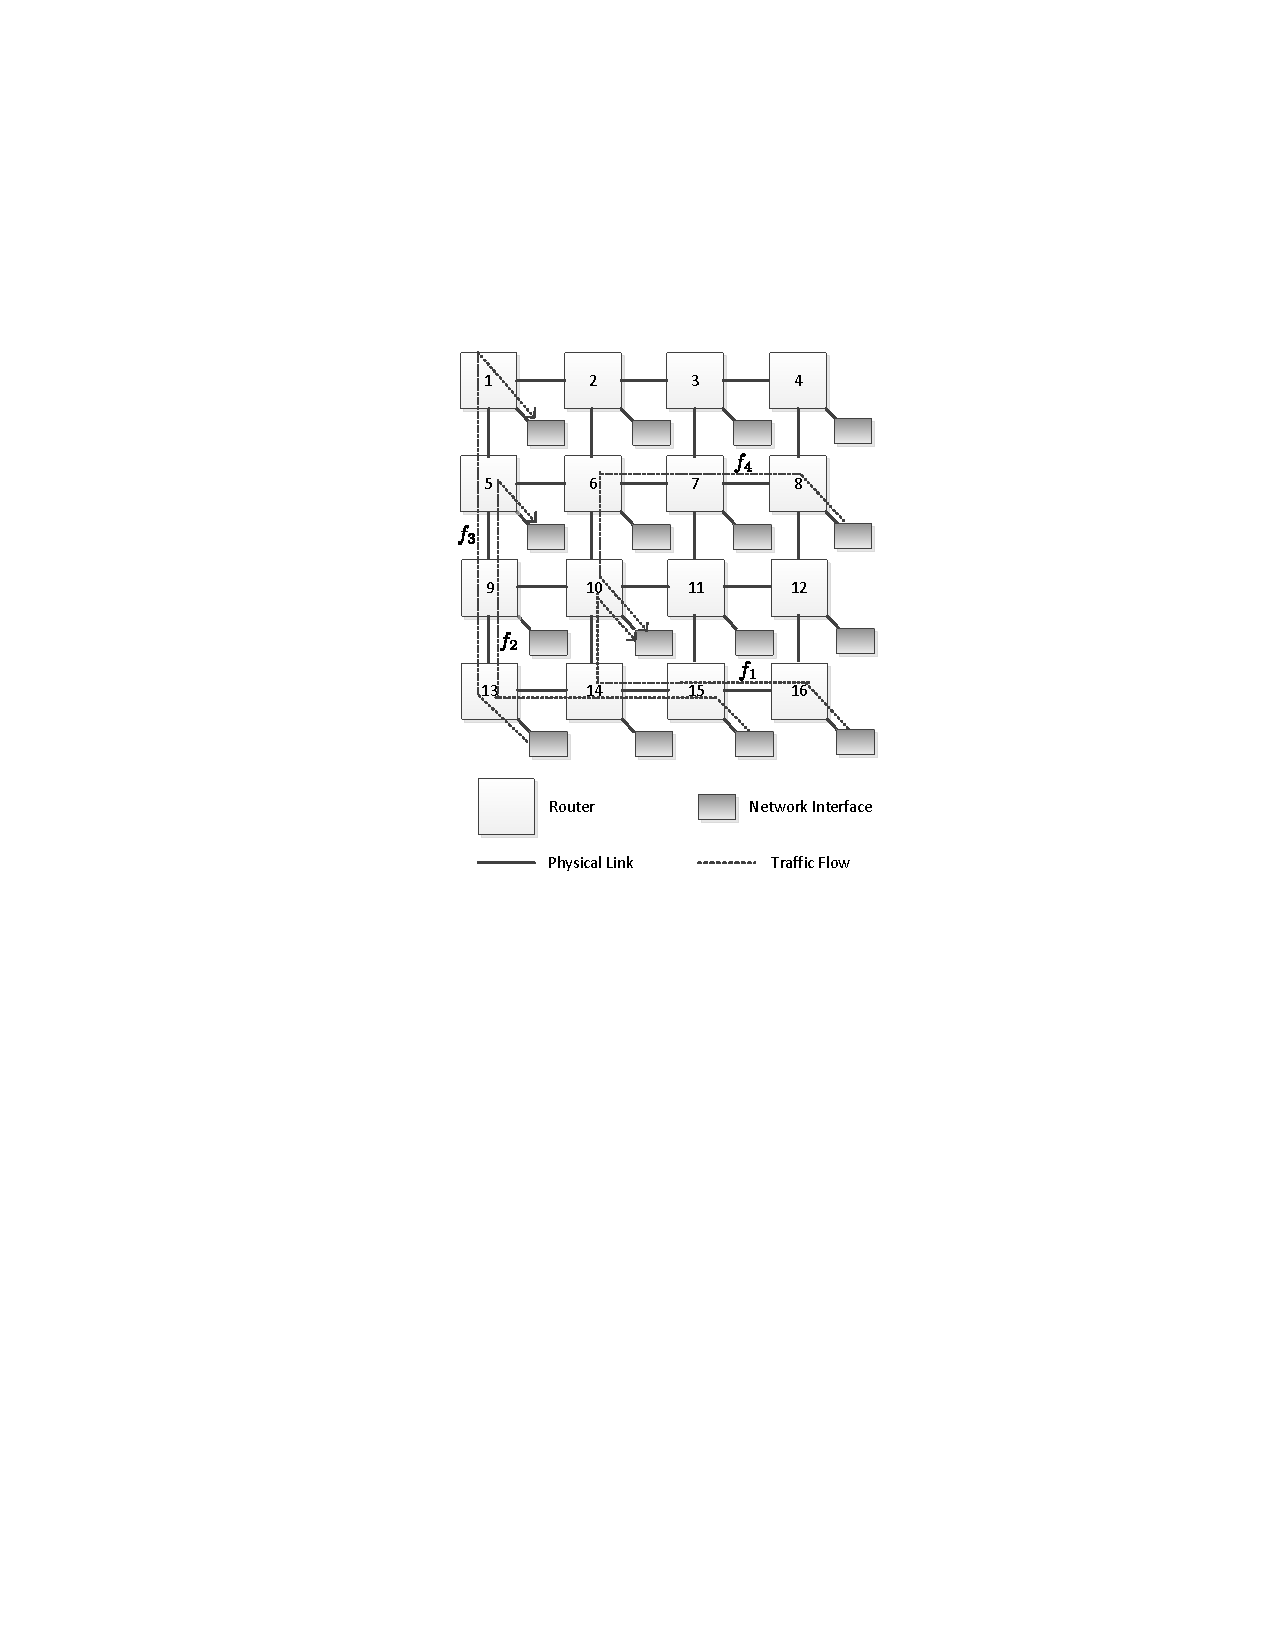
\includegraphics[scale=0.9]{figures/mesh.pdf}\\
  \caption{Mesh topology with 4 real-time traffic flows}\label{topology}
\end{figure}

\subsection{Introduction to Real-Time Calculus}\label{intrortc}
Real-time calculus is an extension of DNC \cite{1253607}, by adding the upper service curve and lower arrival curve to describe the maximal service capacity and lower arrival rate. It is the mathematical basis of Modular Performance Analysis (MPA) \cite{Wandeler2006System} technique used for real-time task scheduling. Here we only present the definition of RTC arrival curve and service curve, for more details about this theory, please refer to \cite{1253607}.
\begin{definition}[Real-Time Arrival Curve \cite{1253607}]
Let $R[s,t)$ denote the number of events that arrived within the time interval $[s,t)$. The lower bound and upper bound on $R[s,t)$ is called the lower arrival curve $\alpha^l$ and upper arrival curve $\alpha^u$, which satisfy
$$\alpha^l(t-s)\leq R[s,t)\leq \alpha^u(t-s),\forall s<t$$
where $\alpha^l(0)=\alpha^u(0)=0$. The RTC arrival curve for $R$ is denoted as $<\alpha^l,\alpha^u>$ for short.
\end{definition}

From the definition, we find that the upper arrival curve (corresponding to the arrival curve of DNC \cite{Boudec2001Network}) and lower arrival curve are used to characterize the upper and lower bound of arrived events within any time interval $\Delta$.

\begin{definition}[Real-Time Service Curve \cite{1253607}]
Let $S[s,t)$ denote the total number of events that can be processed by the system in the time interval $[s,t)$. The lower bound and upper bound on $S[s,t)$ is called the lower service curve $\beta^l$ and upper service curve $\beta^u$, which satisfy
$$\beta^l(t-s)\leq S[s,t)\leq \beta^u(t-s),\forall s<t$$
where $\beta^l(0)=\beta^u(0)=0$. The RTC service curve for $S$ is denoted as $<\beta^l,\beta^u>$ for short.
\end{definition}

From the definition of RTC service curve, we find that the upper and lower service curve are corresponding to the maximal service curve and service curve in DNC theory \cite{Boudec2001Network}, respectively. Thus, the concatenation theorem for service curve (see Theorem 1.46 in \cite{Boudec2001Network}) and maximal service curve (see Theorem 1.6.1 in \cite{Boudec2001Network}) can also be applied to RTC service curve. In this paper, we will use the discrete time RTC arrival curve and service curve to characterize the arrived traffic and service capacity, since the minimal time unit in the wormhole-switched NoC is clock period $T$. Events in arrival curve and service curve refer to the arrival and service of flits, respectively. If we obtain the arrival curve $<\alpha^l,\alpha^u>$ of a specific traffic flow and the service curve $<\beta^l,\beta^u>$ provided to this flow, we can get the output arrival curve $<\alpha^{l^\prime},\alpha^{u^\prime}>$ of this flow and leftover service curve $<\beta^{l^\prime},\beta^{u^\prime}>$ for the other flows with the following equations \cite{1253607}:
\begin{equation}\label{alphal}
\alpha^{l^\prime}=\min\{(\alpha^l\oslash\beta^u)\otimes\beta^l,\beta^l\}
\end{equation}
\begin{equation}\label{alphau}
\alpha^{u^\prime}=\min\{(\alpha^u\otimes\beta^u)\oslash\beta^l,\beta^u\}
\end{equation}
\begin{equation}\label{betal}
\beta^{l^\prime}=(\beta^l-\alpha^u)\bar{\otimes}0
\end{equation}
\begin{equation}\label{betau}
\beta^{u^\prime}=\max\{(\beta^u-\alpha^l)\bar{\oslash}0,0\}
\end{equation}
where $\lceil\cdot\rceil$, $\lfloor\cdot\rfloor$ are the ceiling operator and flooring operator, and $\otimes$, $\oslash$, $\bar{\otimes}$, $\bar{\oslash}$ are corresponding to the min-plus convolution, de-convolution, and max-plus convolution and de-convolution \cite{Boudec2001Network}, respectively.

After we obtained the arrival curve $<\alpha^l_{f_i},\alpha^u_{f_i}>$ of traffic flow $f_i$ and the service curve $<\beta_{R_j,f_i}^l,\beta_{R_j,f_i}^u>$ provided by each router $R_j$ to flow $f_i$ on its path, we can obtain the end-to-end latency and backlog bound by the following equations,
\begin{equation}\label{delay}
Delay(f_i)=H(\alpha^u_{f_i},\beta^l_{R_1,f_i}\otimes\beta^l_{R_2,f_i}\otimes\cdots\otimes\beta^l_{R_N,f_i}),
\end{equation}
\begin{equation}\label{backlog}
Backlog(f_i)=V(\alpha^u_{f_i},\beta^l_{R_1,f_i}\otimes\beta^l_{R_2,f_i}\otimes\cdots\otimes\beta^l_{R_N,f_i})
\end{equation}
where $H(\cdot,\cdot)$ and $V(\cdot,\cdot)$ mean the maximal vertical and horizontal deviation, respectively.

\section{Delay Analysis and Buffer Optimization}\label{modeling}
In this section, we first build the RTC model for the priority-aware NoC. This model consists of two parts, i.e. traffic model and service model. We will introduce two method to obtain the traffic model in subsection \ref{traffic}. The service model is complicated, and the follow four aspects should be considered while constructing the service model for priority-aware NoC: (1) Only head flit need to be processed by RC and VA stage, the subsequent flits of a packet just follow the decision of head flit. We need specific mechanism to characterize the service provided to head and non-head flits in a unified way, so that we can simplify our RTC model. (2) Our model extends the existing approach \cite{73}\cite{Qian489900} by allowing priority sharing between flows. Thus, the leftover service curve provided to lower priority flows can only be derived after all the flows with higher priority have been serviced. (3) Due to the on-chip buffer limitation, credit-based flow control is used as a back-pressure mechanism to prevent buffer overflow. Before analysis the end-to-end performance with Eq.(\ref{delay}) and Eq.(\ref{backlog}), we should first break the cyclic-dependence caused by flow control. (4) To guarantee the tightness of our theoretical bound and simplify the computation, we should collapse the collapsible sub-paths as far as possible. We will discuss the first two issues in subsection \ref{router}, and the last two issues are discussed in subsection \ref{flowcontrol} and subsection \ref{csp}, respectively. Based on the constructed RTC model, we propose a end-to-end latency analysis algorithm and a buffer optimization algorithm. We will introduce these two algorithms in subsection \ref{e2elatency} and subsection \ref{bufferopt}, respectively.

\subsection{Traffic Model}\label{traffic}
In a NoC connected CMP or SoC system, the communication between each pair of IP cores was realized by transmitting packets, and the packet is further divided into flits, which is the minimum transmission unit in wormhole-switched NoC. Denote $<\alpha^l(\Delta),\alpha^u(\Delta)>$ the arrival curve of a flow, we can extract the arrival curve from the synthetic traffic or communication trace with the sliding window method \cite{1253607}. For each window size $\Delta$, this method tries to find the maximal and minimal number of arrived flits (corresponding to $\alpha^l(\Delta)$ and $\alpha^u(\Delta)$) by analyzing the time series of flits. The obtained arrival curve obtained by this method might not be periodic, but, it does not prevent the application of RTC theory. As has been presented in subsection \ref{intrortc}, the service model considered in this paper is a flit-by-flit system. To obtain the worst-case end-to-end packet latency, the obtained arrival curve must be $L$-packetized \cite{Boudec2001Network}. Denote $L_{max}$ the maximum packet length (in flits), $R(t)$ the accumulative arrival function, and $\mathcal{P}^L(\cdot)$ the $L$-packetizer operator, we have
$$R(t)-l_{max}\leq \mathcal{P}^L(R(t))<R(t)$$
and
$$R(s)-l_{max}\leq \mathcal{P}^L(R(s))<R(s)$$
which indicate
$$\alpha(t-s)^l-l_{max}<\mathcal{P}^L(R(t))-\mathcal{P}^L(R(s))<\alpha(t-s)^u+l_{max}.$$
The inequalities above indicate that, if a flow has an arrival curve $<\alpha^l(\Delta),\alpha^u(\Delta)>$, the $L$-packetized flow has a arrival curve $<\alpha^l(\Delta)-l_{max}1_{\{\Delta>0\}},\alpha^u(\Delta)+l_{max}1_{\{\Delta>0\}}>$\footnote{indicator function $1_{\{val\}}$ is equal to 1 if and only if $val$ is true.}. For some special cases, we can directly obtain the $L$-packetized arrival curve instead of transformation from flit arrival curve. Suppose all the packets have the same length $F$ and arrived periodically with period $I$. Then, the service curve of this flow can be obtained by simply amplifying the arrival curve for periodic event stream provided in \cite{1253607} at $y$-axis with a factor $F$, as shown in Fig. \ref{ac}. The alert readers would notice that, the flit arrival curve obtained by this way is also $L$-packetized arrival curve $\mathcal{P}^L(\alpha)$, which can be used to compute the end-to-end packet latency directly.
\begin{figure}
  \centering
  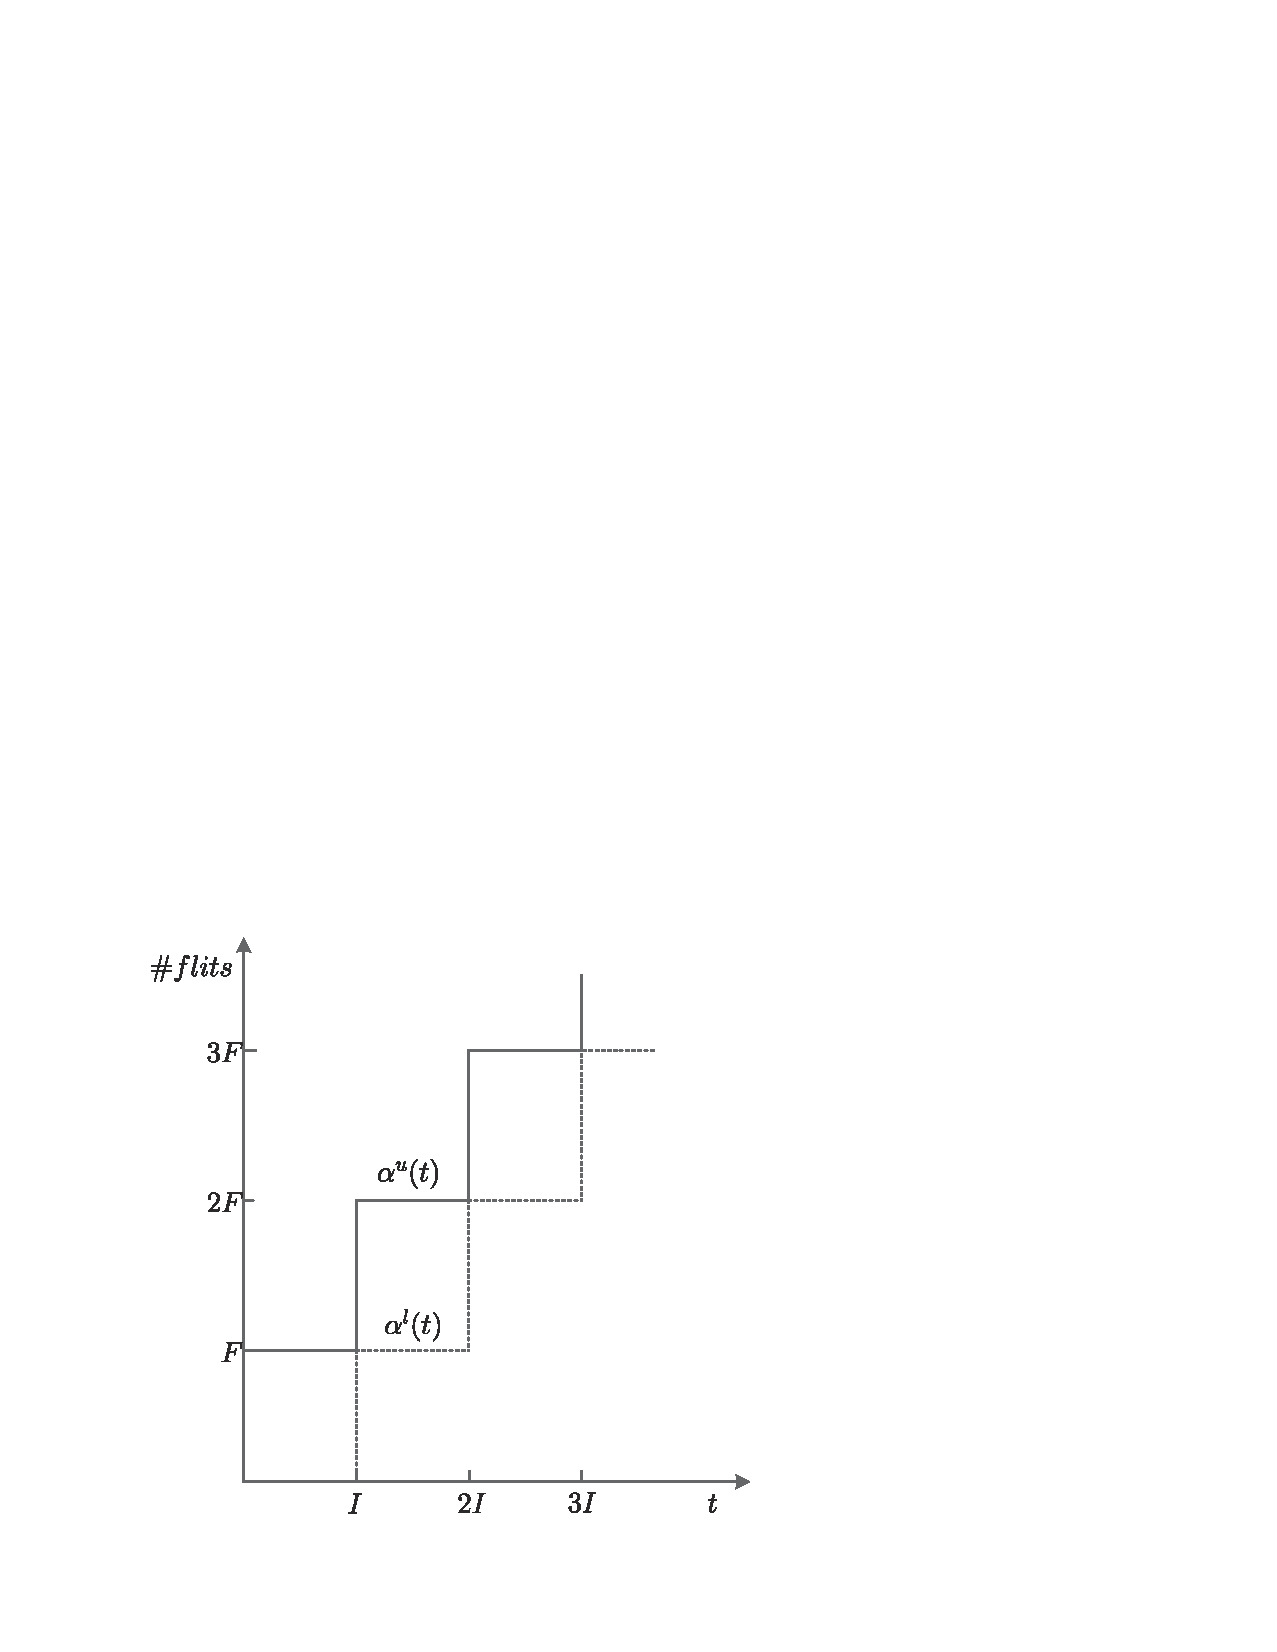
\includegraphics[scale=0.5]{figures/AC.pdf}
  \caption{Real-time calculus arrival curve for periodically arrived traffic with period $I$ and packet length $F$. The solid line and dotted line represent the upper arrival curve and lower arrival curve, respectively.}\label{ac}
\end{figure}

\subsection{Router Model}\label{router}
While modeling the routers with RTC, we can analyze the data path stage-by-stage. After found the service curve for each stage, the service curve provided by the entire router to each flow can be obtained by concatenating all the service curves of these five stages. This is significantly different with the existing DNC based model \cite{qian2009analysis,Qian489900}, where they treat the entire router as a whole and designate a Latency-Rate (LR) service curve for simplicity. The advantage of our method is that, it can be easily modified to characterize the non-standard router micro-architectures, by simply letting the service capacity of non-existing stages to be infinity. Next, we try to obtain the service curves of all these 5 stages:
\begin{figure*}
  \centering
  \subfloat[Service curve of BW, SA and ST stages]{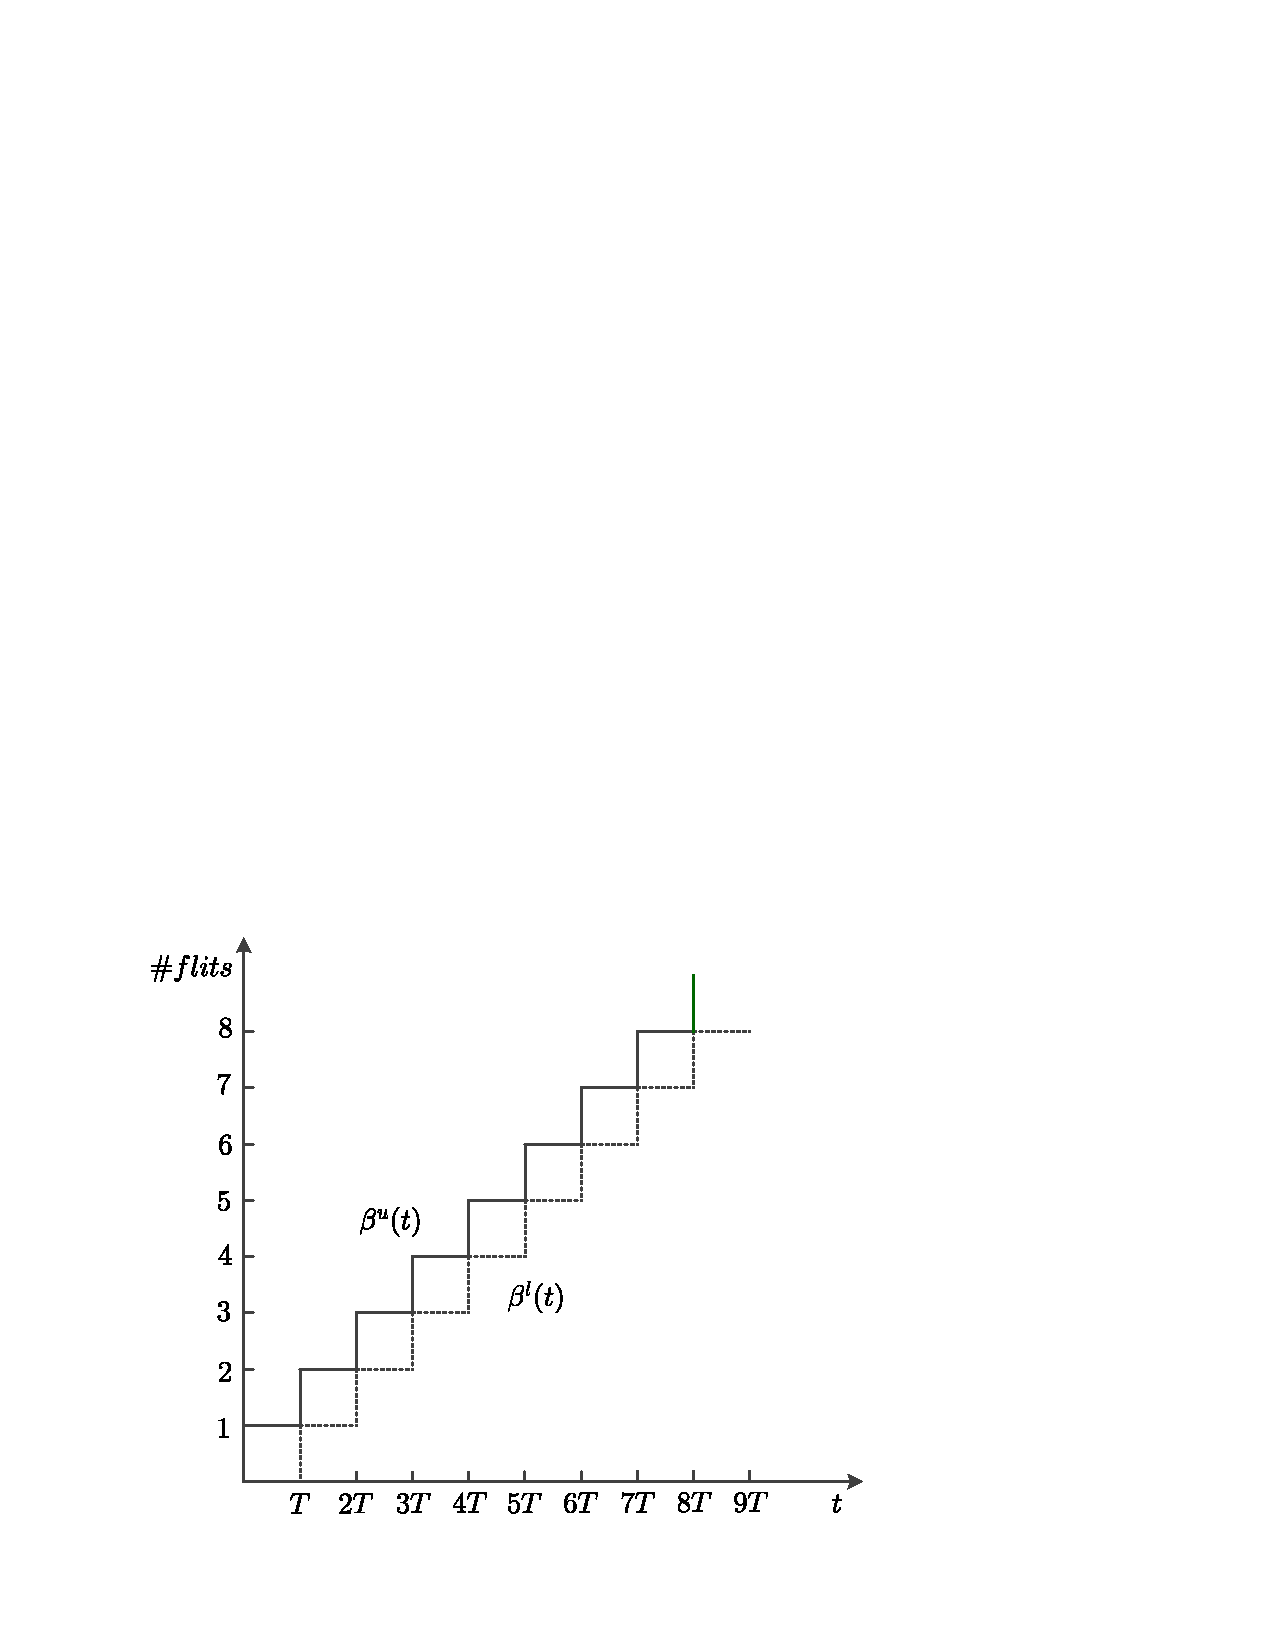
\includegraphics[scale=0.5]{figures/BW_ST_SA.pdf}\label{result1}}\hspace{10pt}
  \subfloat[Service curve of RC and VA stages]{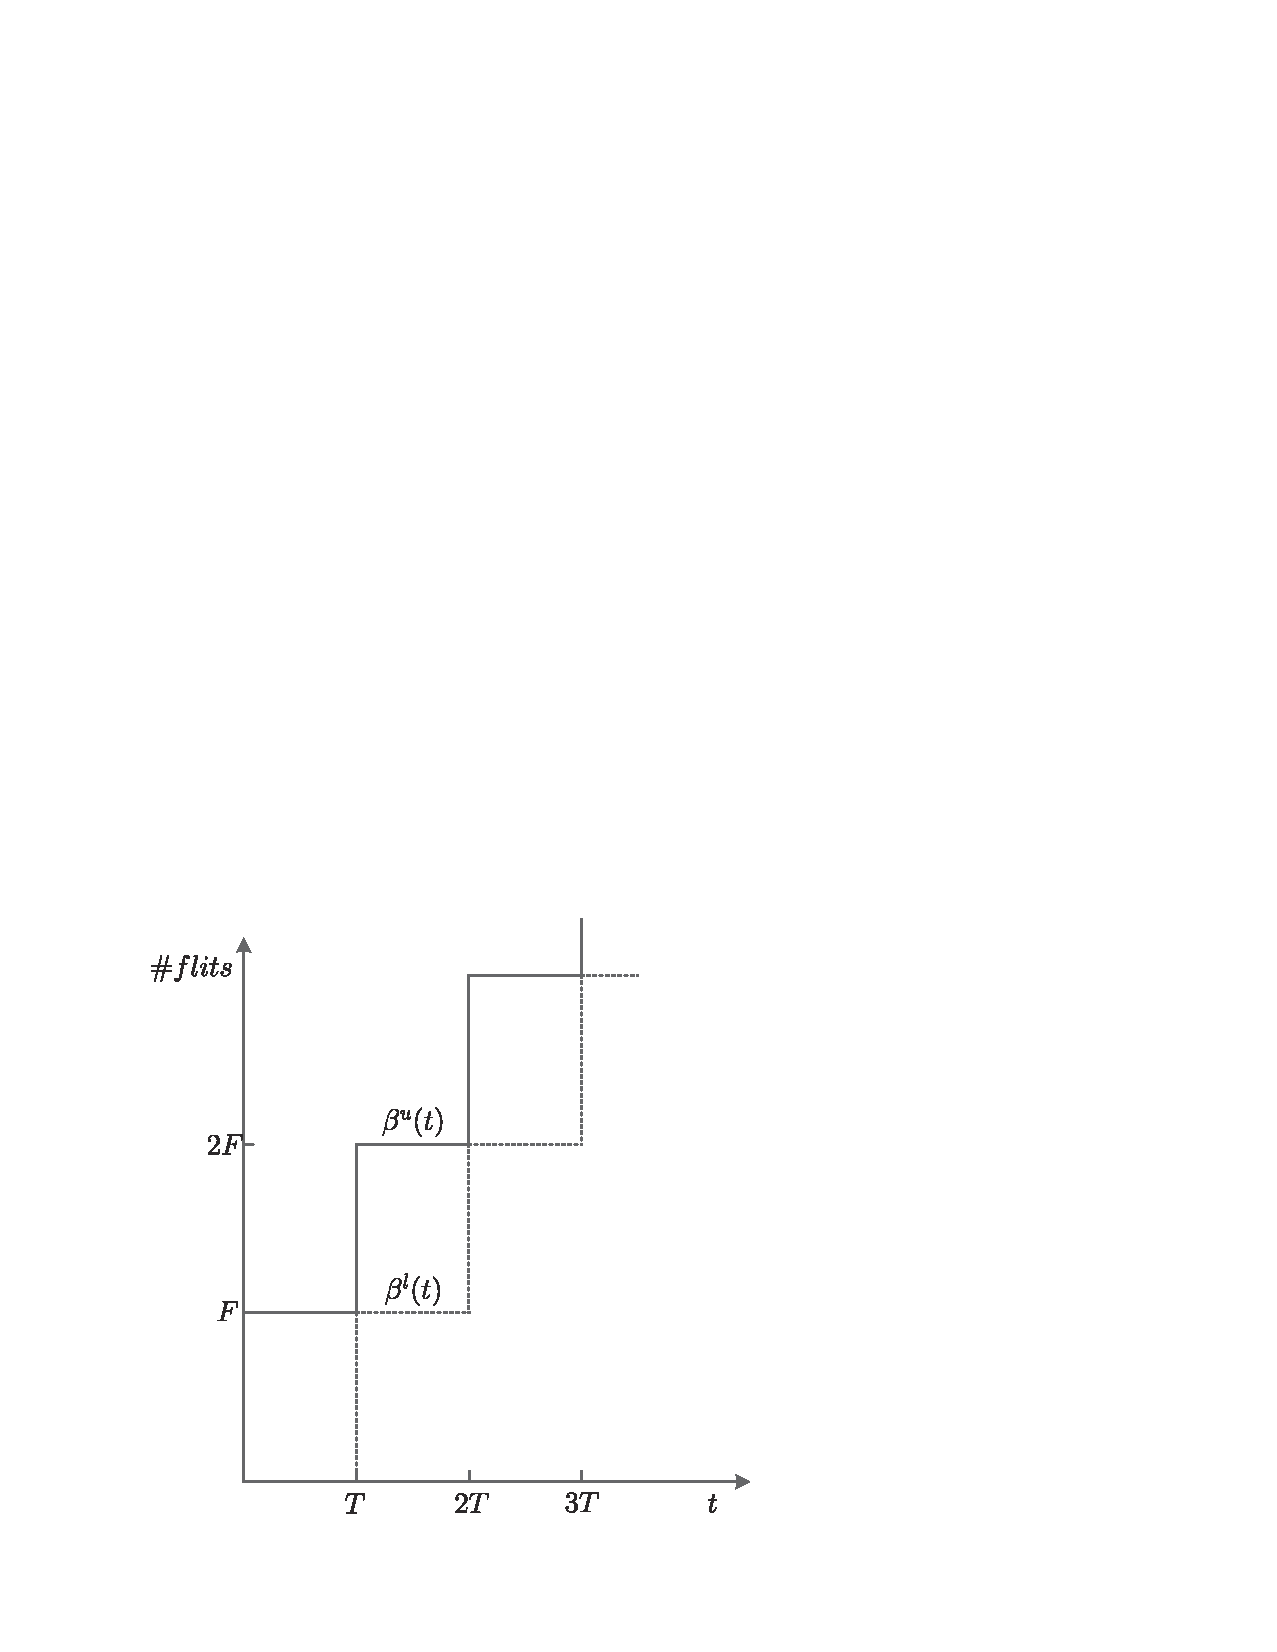
\includegraphics[scale=0.5]{figures/RC_VA.pdf}\label{result2}}
  \caption{Service model for each pipeline stages. The solid lines and dotted lines represent the upper service curves and lower service curves, respectively.}
\end{figure*}

(1) BW stage and ST stage: all the flits within a traffic flow will traverse these two stages, and experience a fixed delay $T$. Take the BW stage as an example, for any time interval of length less than $T$, the maximum and minimal number of flits that can be seen are one and zero, respectively, since it outputs one flit at each cycle $T$. Similarly, for any time interval of length greater than $T$, the maximum and minimal number of flits that can be seen are two and one, respectively. The resulted service curves, i.e. $<\beta^l_{BW},\beta^u_{BW}>$ and $<\beta^l_{ST},\beta^u_{ST}>$, are shown in Fig. \ref{result1}.

(2) RC stage and VA stage: the traverse latency of head flit and non-head flits at these two stages are $T$ and 0, respectively. A sophisticated solution to construct a unified service curve for head flit and non-head flits at these two stages is that, we can view these two stages can provide service for the entire packet within $T$ period. Suppose the packet length is $F$, the equivalent service curve for these two stages, i.e. $<\beta^l_{RC},\beta^u_{RC}>$ and $<\beta^l_{VA},\beta^u_{VA}>$, can be easily obtained by amplifying the service curve of Fig. \ref{result1} in $y$-axis with a factor $F$, as shown in Fig. \ref{result2}.

(3) SA stage: each output port in the wormhole-switched NoC has a SA scheduler to schedule the switch traversal at each cycle. Thus, following the same approach as BW and ST stage, we can get the service curve $<\beta_{SA}^l,\beta_{SA}^u>$ provided by SA stage to all the contention flows, as shown in Fig. \ref{roundrobin}a. For the fixed-priority based scheduling policy, switch allocators provide service for high priority flows first, and flows with the same priority will be served with Round-Robin order. The unserved flows will be imposed an additional latency $T$ due the failure of switch arbitration.

Denote by $<\beta_{SA,R_i,f_j}^l,\beta_{SA,R_i,f_j}^u>$ the service curve provided to flow $f_j$ by SA stage of router $R_i$, the equivalent service curve of router $R_i$ provided to $f_j$, i.e. $<\beta_{R_i,f_j}^l,\beta_{R_i,f_j}^u>$, can be obtained by concatenating the service curves of all the 5 stages together:
$$\beta_{R_i,f_j}^l=\beta_{BW}^l\otimes\beta_{RC}^l\otimes\beta_{VA}^l\otimes\beta_{SA,R_i,f_j}^l\otimes \beta_{ST}^l,$$
$$\beta_{R_i,f_j}^u=\beta_{BW}^u\otimes\beta_{RC}^u\otimes\beta_{VA}^u\otimes\beta_{SA,R_i,f_j}^u\otimes \beta_{ST}^u.$$

The alert readers would notice that, the contention of different flows only occurs at SA stage. Thus, if we obtained the service curve provided by SA stage to flow $f_j$, we can obtain the service curve of router directly. Suppose the leftover service curve after serving flows with high priority than $f_j$ is $<\beta_{SA,R_i}^{l^\prime},\beta_{SA,R_i}^{u^\prime}>$, to obtain the service curve $<\beta_{SA,R_i,f_j}^l,\beta_{SA,R_i,f_j}^u>$, we should consider the following two cases:

(a) all the flows contending with $f_j$ at $R_i$ have lower priorities. For the synchronize router architecture, flow $f_j$ obtain the total leftover service curve $<\beta_{SA,R_i}^{l^\prime},\beta_{SA,R_i}^{u^\prime}>$. But for an asynchronous architecture, we should take the inference from low-priority flows into consideration. For example, a flit from $f_j$ arriving at SA stage just after a flit from lower priority gotten granted has to stall for a cycle. At this circumstance, the actual service curve obtained by flow $f_j$ is
\begin{equation}\label{nonpreemptbetal}
\beta^{l}_{SA,R_i,f_j}=\max\{0,\beta^{l^\prime}_{SA,R_i}-1\}
\end{equation}
where $\beta^{l^\prime}_{SA,R_i,f_j}$ is the leftover service curve calculated with Eq.(\ref{betal}). Similarly, a flow with higher priority than $f_j$ can also be blocked by $f_j$ for a cycle. Thus, denote by $\beta^{u^\prime}_{SA,R_i,f_j}$ the service curve calculated with Eq.(\ref{betau}), the actual upper service curve obtained by flow $f_j$ is
\begin{equation}\label{nonpreemptbetau}
\beta^{u}_{SA,R_i,f_j}=\min\{\beta^{u}_{SA,R_i,f_j},\beta^{u^\prime}_{SA,R_i}+1\}.
\end{equation}

(b) there exists some contention flows with the same priority as $f_j$. Denote by the set of contention flows at router $R_i$ with the same priority as $f_j$ as $\Theta_{R_i,f_j}$, and let $N_{R_i,f_j}$ be the number of flows in $\Theta_{R_i,f_j}$. Then, the service curve provided to $f_j$ is $<\lfloor\beta^{l^\prime}_{SA,R_i}/(N_{R_i,f_j}+1)\rfloor,\lceil\beta^{u^\prime}_{SA,R_i}/(N_{R_i,f_j}+1)\rceil>$, since all the flows in $\Theta_{R_i,f_j}$ got service in Round-Robin order. This is slightly different from the conventional continuous time model which is $<\beta^{l^\prime}_{SA,R_i}/(N_{R_i,f_j}+1),\beta^{u^\prime}_{SA,R_i}/(N_{R_i,f_j}+1)>$, because our model is flit-level preemptive. An example with two flows with the same priority is shown in Fig. \ref{roundrobin}. After serving by all the flows in $\Theta_{R_i,f_j}$, the leftover service capacity for low priority flows can be obtained by applying Eq.(\ref{betal}) and Eq.(\ref{betau}).
\begin{figure*}
  \centering
  % Requires \usepackage{graphicx}
  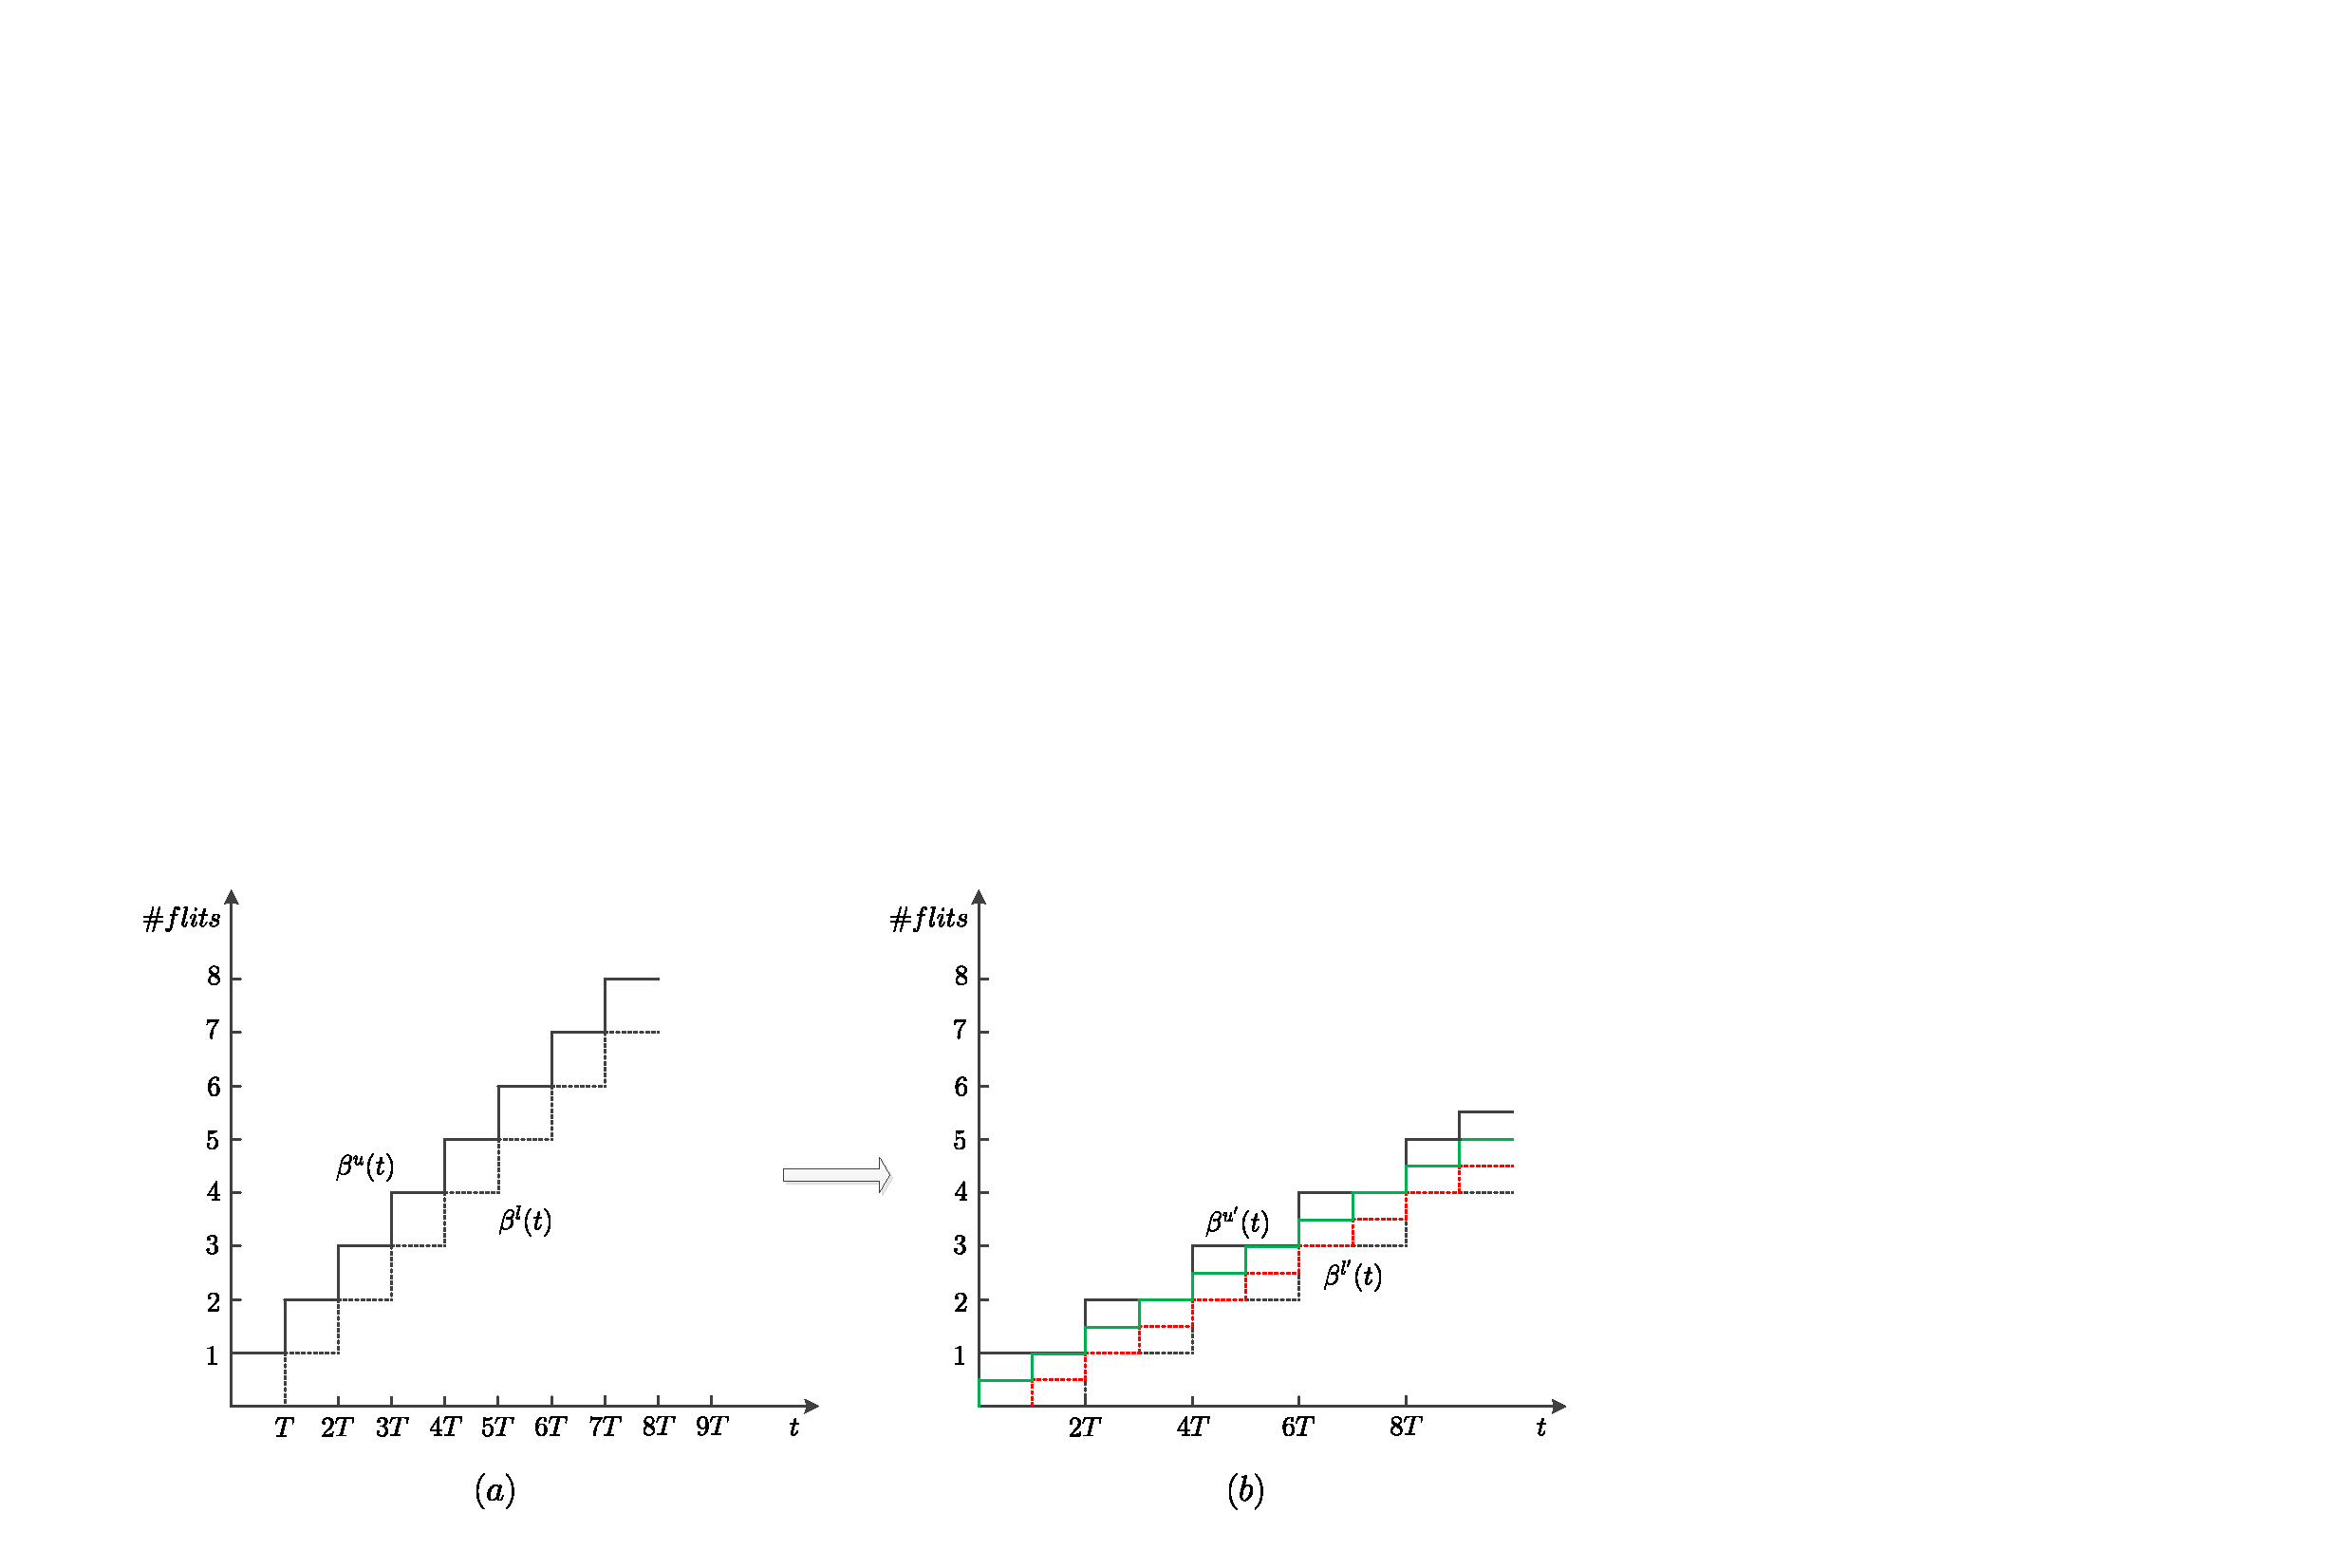
\includegraphics[scale=0.5]{figures/RoundRobin.pdf}\\
  \caption{Service curve of SA stage for two flows with the same priority under Round-Robin scheduling policy. (a) Service capacity of SA stage. (b) Upper and lower service curve provided to each contending flow, corresponding to the solid line and dotted line; the solid green line and dotted red line represent the unrounded upper and lower service curves.}\label{roundrobin}
\end{figure*}

\subsection{Upper Service Curve for Flow Controller}\label{flowcontrol}
Credit-based flow control introduces cyclic-dependence between the adjacent routers, and leads to the self-blocking within a flow due to the insufficiency of buffer space at the downstream router. Historically, the effect of self-blocking is computed numerically by fixed-point iteration \cite{schioler2005network} or symbolically analyzed by the transformation from marked dataflow graph \cite{Thiele:2009:MPA:1629335.1629353}. In this paper, we try to tackle the same problem with another solution. This is motivated by \cite{qian2009analysis}, where the authors abstract the flow control as a network element (called flow controller) providing a service curve $\beta_{\tau}$ (corresponding to the lower service curve $\beta_\tau^l$ of RTC), which can be obtained by applying some basic properties of dioid algebra. In this section, we follow the same procedure in \cite{qian2009analysis} to derive the upper service curve of flow controller. The obtained upper service curve together with the lower service curve derived in \cite{qian2009analysis} enables us to break the control loop caused by flow control and build a comprehensive performance model with RTC. To make the question clear, we take flow $f_2$ as an example to demonstrate this method. The scheduling network of flow $f_2$ is plotted in Fig. \ref{f2}, we ignore flow $f_4$ and the flow control of other flows for simplicity. We assume that, the destination IP core can consume the ejected flits immediately, thus there is no flow controller between the ejection router and destination NI. But, to prevent the buffer overflow, there must be a flow controller between input NI and injection router. We try to derive the upper service curve of flow controller at router $R_9$, as shown in the following Theorem.
\begin{figure*}
  \centering
  % Requires \usepackage{graphicx}
  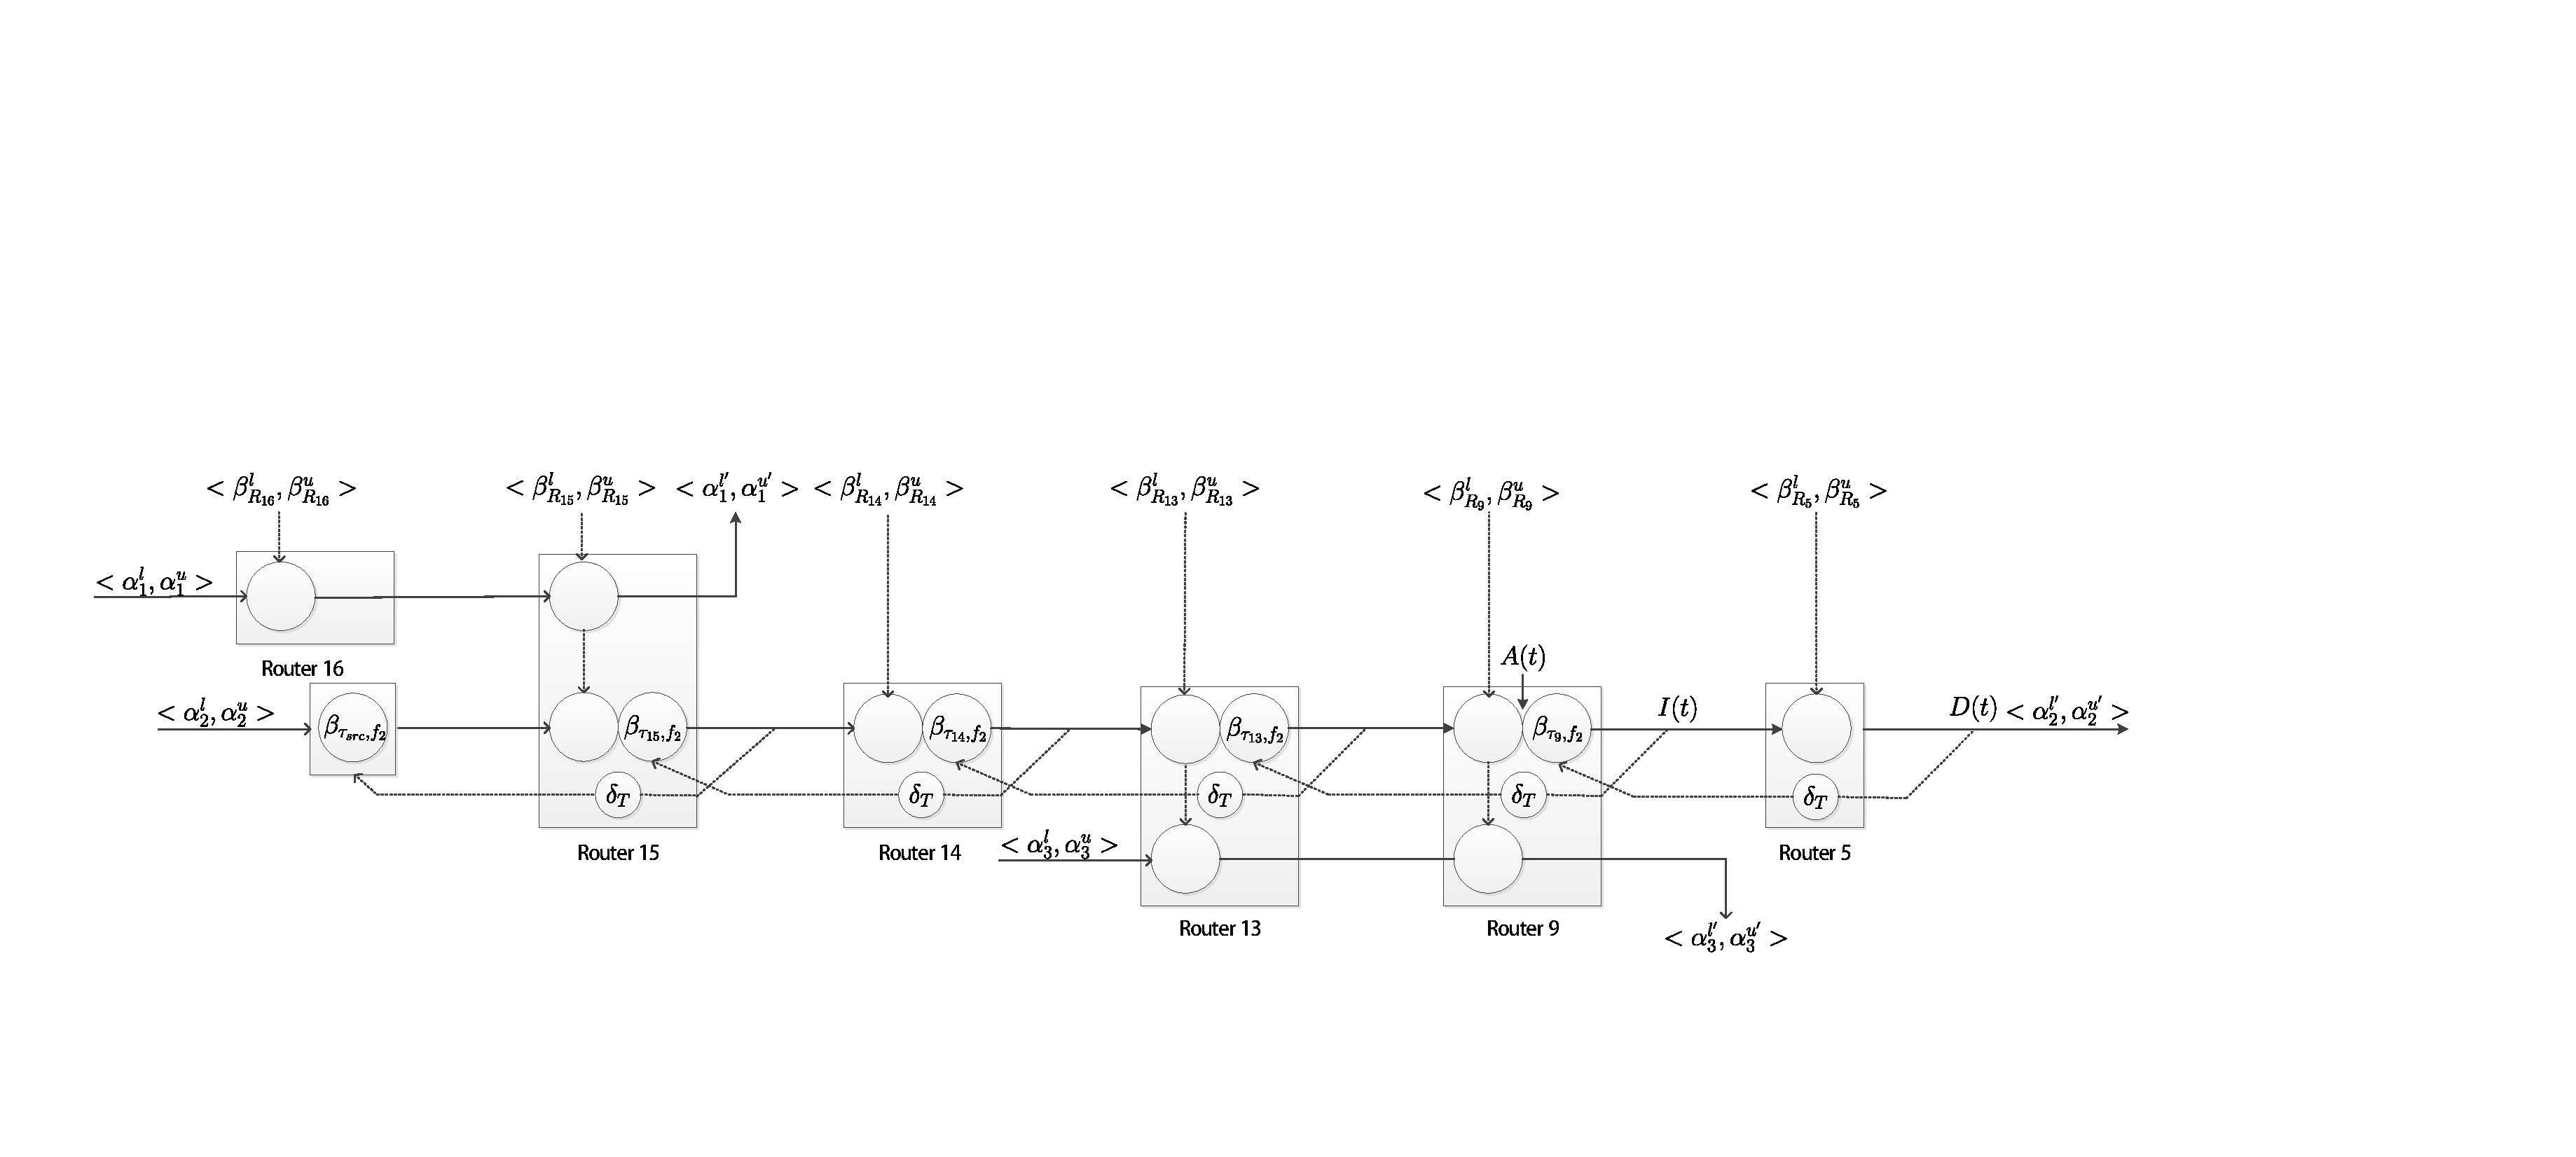
\includegraphics[scale=0.35]{figures/f2.pdf}\\
  \caption{Scheduling network model for flow $f_2$}\label{f2}
\end{figure*}

\begin{theorem}\label{credit}
Suppose the router provides an upper service curve $\beta^u$, the buffer size and credit feedback delay are denoted as $B$ and $\sigma$. Then the flow controller provides an equivalent upper service curve $$\beta^{u}_\tau(t)=\overline{\beta^u\otimes\delta_\sigma(t)+B}$$ where $\bar{f}$ is the sub-additive closure of $f$ \cite{Boudec2001Network} and $\delta_\sigma(t)=+\infty$ for $\forall t>\sigma$, otherwise $\delta_\sigma(t)=0$.
\end{theorem}
\begin{IEEEproof}
We take the flow control between $R_9$ and $R_5$ in Fig. \ref{f2} as an example to proof this theorem. Denote the amount of injected and departed flits at $R_5$ by time $t$ as $I(t)$ and $D(t)$, the amount of flits served by $R_9$ as $A(t)$. The feedback link can be represented as a network element providing upper service curve $\delta_\sigma(t)$. Next, we apply the basic properties of service curve and dioid algebra to derive the upper service curve this flow controller. We have $I(t)=\min\{A(t),D^\prime(t)+B\}$ by the property of credit-based flow control, where $D^\prime=D\otimes\delta_\sigma$.

Based on property of upper service curve $\beta^u$, we have\footnote{An alternative definition of upper service curve, see definition 1.6.1 in \cite{Boudec2001Network} for more details.}
$$D(t)\leq I\otimes \beta^u(t).$$

Bring $I(t)$ and $D^\prime(t)$ into this equality, we get
\begin{eqnarray*}
D(t)&\leq& I\otimes \beta^u(t)\\
&\leq& \min\{A\otimes \beta^u(t),D\otimes\delta_\sigma\otimes \beta^u(t)+B\}.
\end{eqnarray*}
By applying Theorem 4.31 in \cite{Boudec2001Network}, we have
$$D\leq A\otimes \beta^u\otimes\overline{\beta^u\otimes\delta_\sigma+B}.$$
Thus,
\begin{eqnarray*}
  I&=& \min\{A,D^\prime+B\}\\
  &\leq& \min\{A,D\otimes\delta_\sigma+B\}\\
  &\leq& \min\{A,A\otimes \beta^u\otimes\overline{\beta^u\otimes\delta_\sigma+B}\otimes\delta_\sigma+B\}\\
  &=& \min\{A\otimes \delta_\sigma,A\otimes (\beta^u\otimes\delta_\sigma+B)\otimes\overline{\delta_\sigma\otimes\beta^u+B}\}\\
  &=& \min\{A\otimes \delta_\sigma,A\otimes \overline{\delta_\sigma\otimes\beta^u+B}\}\\
  &=& A\otimes\min\{\delta_\sigma,\overline{\beta^u\otimes\delta_\sigma+B}\}\\
  &=& A\otimes\overline{\beta^u\otimes\delta_\sigma+B}.
\end{eqnarray*}
which implies that, the flow controller has an equivalent upper service curve $\overline{\beta^u\otimes\delta_\sigma+B}$.
\end{IEEEproof}

Theorem \ref{credit} derives the upper service curve of a single flow controller, and we can get the service curves of all the flow controllers along the router chain of all the flows by applying Theorem \ref{credit} iteratively. As shown in Fig. \ref{f2}, the service curve of downstream routers can affect the service curve of flow controller at upstream. Hence, we should compute the service curves of flow controller from destination to source. Take flow $f_2$ as an example, we should first derive the service curves of $f_2$ obtained at each router with the method provided in Subsection \ref{router}. Service curve obtained at Router $R_{15}$ to flow $f_2$ can be derived by applying Eq.(\ref{betal}) and Eq.(\ref{betau}), since $f_2$ is a lower priority flow at $R_{15}$. Router $R_{13}$, $R_{9}$ and $R_{5}$ provide all their service capacity to $f_2$ because $f_2$ is the highest priority flow at these routers. Then, the service curve of flow controller at router $R_{9}$ can be obtained by applying Theorem \ref{credit}, which is $<\beta_{\tau_9}^l,\beta_{\tau_9}^u>$. By applying the concatenation theorem, we can obtain the equivalent service curve of router $R_{9}$ are $<\beta_{R_9}^l\otimes\beta_{\tau_9}^l,\beta_{R_9}^u\otimes\beta_{\tau_9}^u>$. Follow the same procedure, we can get the service curve of flow controller at router $R_{13}$, $R_{14}$, $R_{15}$ and NI that connected to $R_{15}$ iteratively.

\subsection{Collapsible Sub-Path}\label{csp}
We have build the traffic model, router model and flow control model in the previous subsections. Before giving the performance evaluation algorithm, we first consider the follow scenario. Take $f_2$ and $f_3$ in Fig. \ref{topology} as an example, they content the output link at both router $R_{13}$ and $R_{9}$. Suppose $P_2>P_3$ and denote by $B_{R_9,f_2}$ the buffer size of $R_{9}$ allocated to flow $f_2$, $<\beta_{R_{13},f_2}^l,\beta_{R_{13},f_2}^u>$ and $<\beta_{R_{9},f_2}^l,\beta_{R_{9},f_2}^u>$ the service curve of $R_{13}$ and $R_{9}$ provided to flow $f_2$, $<\beta_{\tau_{13},f_2}^l,\beta_{\tau_{13},f_2}^u>$ the service curve for flow controller of router $R_{13}$, $<\alpha_{R_{13},f_2}^l,\alpha_{R_{13},f_2}^u>$ and $<\alpha_{R_{13},f_3}^l,\alpha_{R_{13},f_3}^u>$ the arrival curve of $f_2$ and $f_3$ at router $R_{13}$. The question is: when $B_{R_9,f_2}$ is sufficiently large so that $\beta_{R_{13},f_2}^l\otimes\beta_{\tau_{13},f_2}^l=\beta_{R_{13},f_2}^l$ and $\beta_{R_{13},f_2}^u\otimes\beta_{\tau_{13},f_2}^u=\beta_{R_{13},f_2}^u$, how to derive the leftover service curve for $f_3$ at $R_{13}$ and $R_9$, and obtain a tight performance bound of $f_3$ efficiently?

An intuitive solution is: Firstly, obtaining the leftover service curve of $R_{13}$ by applying Eq.(\ref{betal}) and Eq.(\ref{betau}); Secondly, deriving the output arrival curve $<\alpha_{R_{9},f_2}^{l^\prime},\alpha_{R_{9},f_2}^{u^\prime}>$ of $f_2$ by applying Eq.(\ref{alphal}) and Eq.(\ref{alphau}); Thirdly, the leftover service curve of $R_9$ can be easily obtained by applying Eq.(\ref{betal}) and Eq.(\ref{betau}); And finally, the leftover service curve for $f_3$ at $R_{13}$ and $R_9$ can be easily obtained by concatenating these two service curves. Another solution is: we can substitute $R_{13}$ and $R_{9}$ by a virtual router $R_{13,9}$ providing service curve $<\beta_{R_{13},f_2}^l\otimes\beta_{R_{13},f_2}^l,\beta_{R_{13},f_2}^u\otimes\beta_{R_{13},f_2}^u>$, since $B_{R_9,f_2}$ is sufficiently large and the flow control between $R_{13}$ and $R_9$ can be ignored, as shown in Fig. \ref{collapse}. Then, the leftover service curve $f_3$ obtained at $R_{13}$ and $R_{9}$ can be directly obtained by applying Eq.(\ref{betal}) and Eq.(\ref{betau}). Compared with previous router-by-router calculation method, it eliminates the calculation of intermediate arrival curve, and compute the equivalent service curve by just invoke Eq.(\ref{betal}) and Eq.(\ref{betau}) once, which is calculation efficient. We formalize this observation and propose the concept of Collapsible Sub-Path (CSP).
\begin{figure}
  \centering
  % Requires \usepackage{graphicx}
  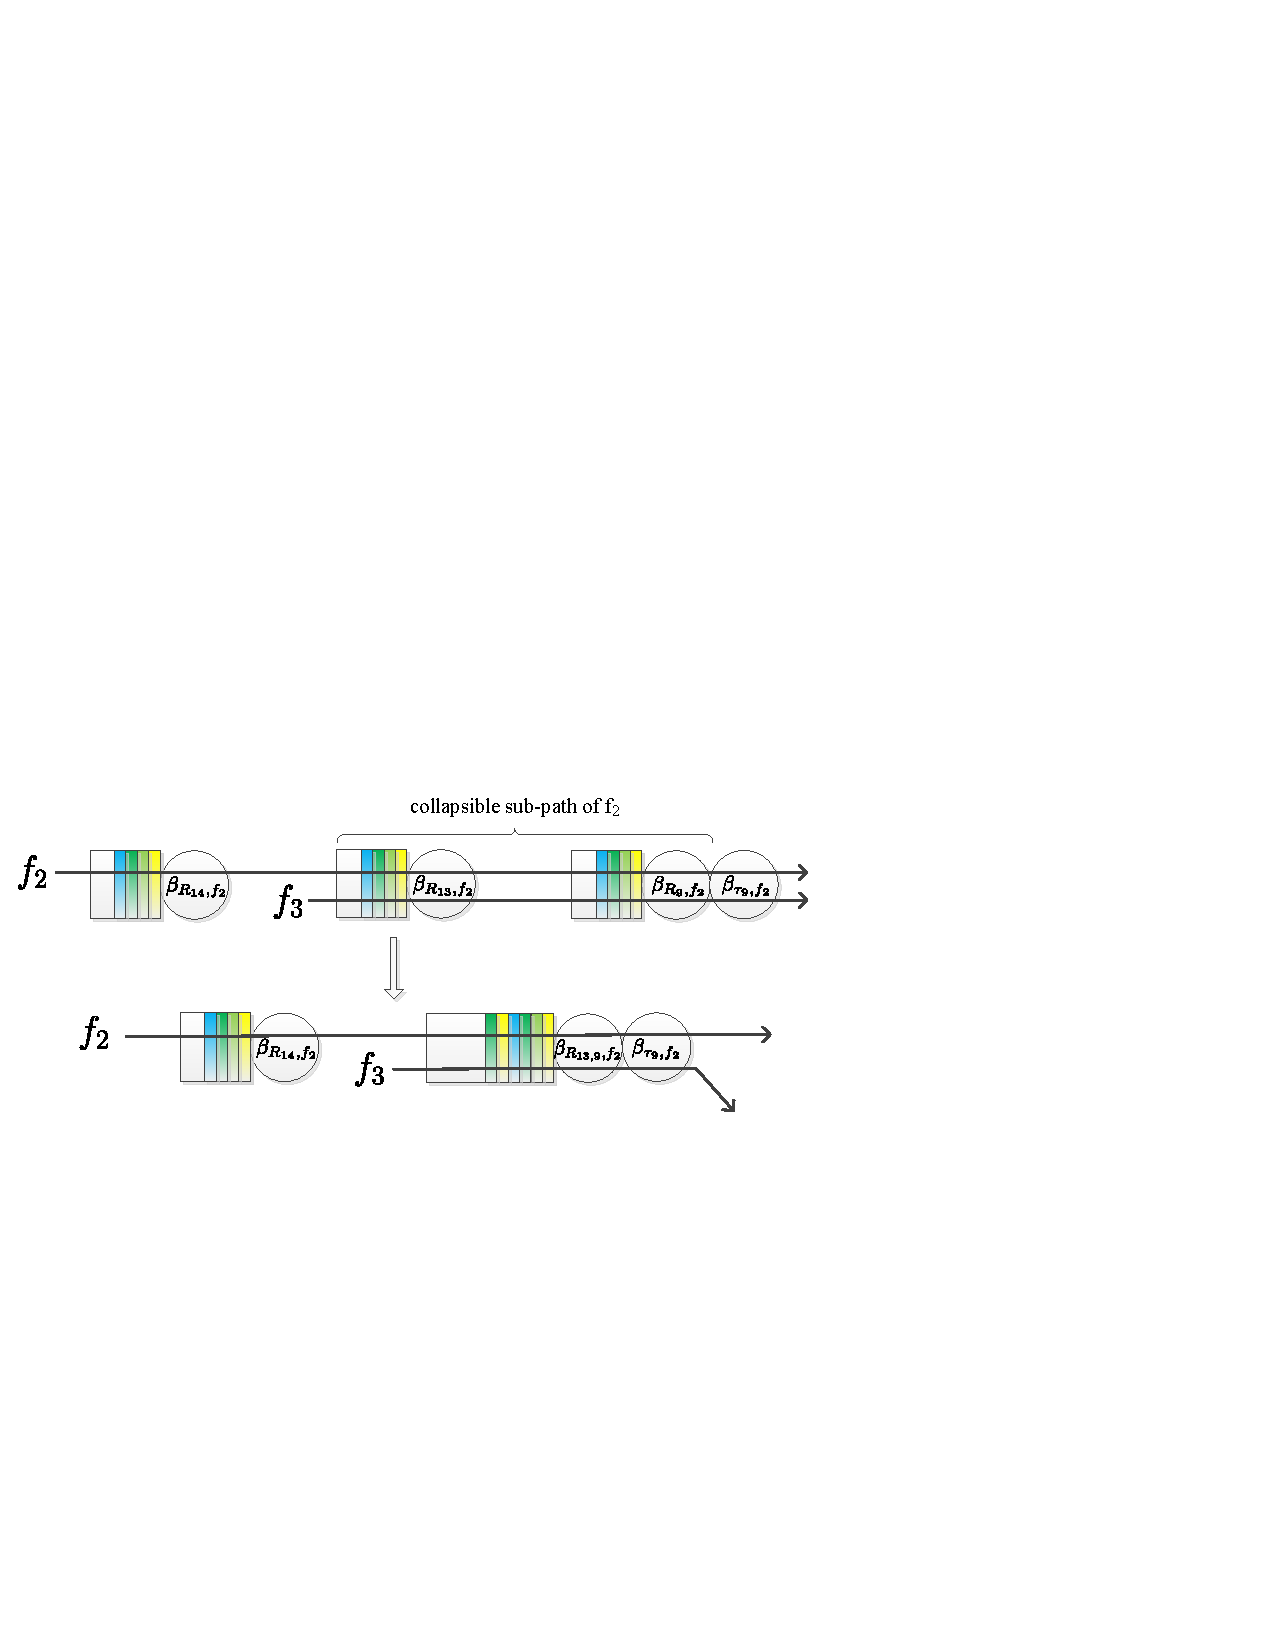
\includegraphics[scale=0.65]{figures/collapse.pdf}\\
  \caption{Collapsible sub-path of $f_2$. Since the flow control between $R_{13}$ and $R_9$ can be ignored, they are replaced by a single virtual router $R_{13,9}$.}\label{collapse}
\end{figure}

\begin{definition}[Collapsible Sub-Path]
The collapsible sub-path of flow $f$, denoted by $CSP(f)$, is a sub-path of $f$ satisfying the follow conditions:
\begin{enumerate}
  \item all the routers $R_i$ on this sub-path, except the last one, satisfy $\beta_{R_{i},f}^l\otimes\beta_{\tau_{i},f}^l=\beta_{R_{i},f}^l$ and $\beta_{R_{i},f}^u\otimes\beta_{\tau_{i},f}^u=\beta_{R_{i},f}^u$.
  \item $CSP(f)$ is also a sub-path of all the flows in $\Omega_{f}$, where $\Omega_{f}$ is the set of contention flows with lower priorities on this sub-path.
\end{enumerate}
\end{definition}

For the high-priority flows, the process of calculating the end-to-end equivalent service curve is also a collapsing process. But, to compute the leftover service curve for low-priority flows at some routers, we have to know the arrival curve of high-priority flows at these routers. As implied previously, instead of the router-by-router calculation, we can leverage the concept of CSP and replace all the routers on $CSP(f)$ with a single virtual router providing service curve $<\otimes_{R_i\in CSP(f)}\beta_{R_i,f}^l,\otimes_{R_i\in CSP(f)}\beta_{R_i,f}^u>$. For a CSP with $n$ ($n\geq 2$) routers, this method reduces $n-1$ times calculation of arrival curve and leftover service curve. The leftover service curve calculation is greatly simplified, and the accuracy of performance bound is also improved due to the well-known ``Pay-Burst-Only-Once" phenomenon in DNC theory \cite{Boudec2001Network}. We will propose our improved latency analysis algorithm in the next subsection, which automatically identifies and collapses all the CSPs on the path of a flow.

\subsection{End-to-End Latency}\label{e2elatency}
After obtained the traffic model, router model and flow control model, compute the end-to-end latency is still a non-trivial task. The follow four aspects should be considered carefully: (1) We should always compute the end-to-end latency by collapsing all the CSP to a single virtual node, as the hop-by-hop computation will lead to a looser bound; (2) In the fixed-priority flit-level preemptive NoC, only the leftover service curve can be used by the low priority flows, thus, our computation must start from higher priority flows to lower priority; (3) Before computing the leftover service curve for lower priority flows, we must ensure that all the higher priority flows has been served; (4) The computed service curve for flow controller can only be applicable for specific flow, and we should compute these curves for each flows. Keeping these four aspects in mind, we propose the performance evaluation algorithm, as shown in Algorithm \ref{alg:equivalentservicecurve}.
\begin{algorithm}
\caption{End-to-End Latency Analysis Algorithm}
\label{alg:equivalentservicecurve}
\begin{algorithmic}[1]
\REQUIRE Scheduling Network
\ENSURE Worst-case End-to-End Latency for all the flows
    \FOR {each flow $f_i\in \mathcal{F}$ with priority order}
        \STATE $\beta_{\tau}^l=\delta_0(t)$; $\beta_{\tau}^u=\delta_0(t)$;
        \FOR {each router $R_j\in \mathcal{R}_{i}$ from $end_i$ to $start_i$}
            \IF {$\Theta_{R_j,f_i}\neq \emptyset$}
                \STATE $\beta_{R_j,f_i}^l=\beta_{BW}^l\otimes\beta_{RC}^l\otimes\beta_{VA}^l\otimes\lfloor\frac{\beta_{SA,R_j}^{l^\prime}}{N_{R_j,f_i}+1}\rfloor\otimes\beta_{ST}^l$;
                \STATE $\beta_{R_j,f_i}^u=\beta_{BW}^u\otimes\beta_{RC}^u\otimes\beta_{VA}^u\otimes\lceil\frac{\beta_{SA,R_j}^{u^\prime}}{N_{R_j,f_i}+1}\rceil\otimes\beta_{ST}^u$;
            \ELSE
                \STATE $\beta_{R_j,f_i}^l=\beta_{BW}^l\otimes\beta_{RC}^l\otimes\beta_{VA}^l\otimes\beta_{SA,R_j}^{l^\prime}\otimes\beta_{ST}^l$;
                \STATE $\beta_{R_j,f_i}^u=\beta_{BW}^u\otimes\beta_{RC}^u\otimes\beta_{VA}^u\otimes\beta_{SA,R_j}^{u^\prime}\otimes\beta_{ST}^u$;
            \ENDIF
            \STATE $\beta^{l}_{\tau_j,f_i}(t)=\beta_{\tau}^l$; $\beta_{\tau}^l=\overline{\beta^l_{R_j,f_i}\otimes\beta^{l}_{\tau}\otimes\delta_\sigma(t)+B_{R_j,f_i}}$;
            \STATE $\beta^{u}_{\tau_j,f_i}(t)=\beta_{\tau}^u$; $\beta_{\tau}^u=\overline{\beta^u_{R_j,f_i}\otimes\beta^{u}_{\tau}\otimes\delta_\sigma(t)+B_{R_j,f_i}}$;
        \ENDFOR
        \STATE Collapse $CSP(f_i)$ and update $\Theta_{R_j,\cdot}$, $\Omega_{R_j,\cdot}$ and $\mathcal{R}_{\cdot}$;
        \STATE $Delay(f_i)=H(\alpha^u_{f_i},\underset{R_k\in\mathcal{R}_{f_i}}{\otimes}(\beta^l_{R_k,f_i}\otimes\beta^l_{\tau_k,f_i}))$;
        \STATE $\beta_{f_i}^l=\delta_0(t)$; $\beta_{f_i}^u=\delta_0(t)$;
        \FOR {For $\forall R_j\in\mathcal{R}_{f_i}$ from $start_i$ to $end_i$}
            \STATE $\beta^l=\beta^l_{f_i}\otimes\beta_{BW}^l\otimes\beta_{RC}^l\otimes\beta_{VA}^l$;
            \STATE $\beta^u=\beta^u_{f_i}\otimes\beta_{BW}^u\otimes\beta_{RC}^u\otimes\beta_{VA}^u$;
            \STATE $\alpha^l_{R_j,f_i}=\min\{(\alpha^l_{f_i}\oslash\beta^u)\otimes\beta^l,\beta^l\}$;
            \STATE $\alpha^u_{R_j,f_i}=\min\{(\alpha^u_{f_i}\otimes\beta^u)\oslash\beta^l,\beta^u\}$;
            \STATE $\beta_{f_i}^l=\beta_{f_i}^l\otimes\beta_{R_j,f_i}^l\otimes\beta^l_{R_j,f_i}$;
            \STATE $\beta_{f_i}^u=\beta_{f_i}^u\otimes\beta_{R_j,f_i}^u\otimes\beta_{R_j,f_i}^u$;
            \IF {$\Omega_{R_j,f_i}\neq \emptyset$}
                \IF {delay of $\forall f_k\in\Theta_{R_j,f_i}$ has been calculated}
                    \STATE $\alpha^l_{R_j,f_i}=\alpha^l_{R_j,f_i}+\sum_{f_k\in\Theta_{R_j,f_i}}\alpha^l_{R_j,f_k}$;
                    \STATE $\alpha^u_{R_j,f_i}=\alpha^u_{R_j,f_i}+\sum_{f_k\in\Theta_{R_j,f_i}}\alpha^u_{R_j,f_k}$;
                \ENDIF
                \STATE $\beta^{l^\prime}_{SA,R_j}=(\beta^{l^\prime}_{SA,R_j}-\alpha^u_{R_j,f_i})\bar{\otimes}0$;
                \STATE $\beta^{u^\prime}_{SA,R_j}=\max\{(\beta^{u^\prime}_{SA,R_j}-\alpha^l_{R_j,f_i})\bar{\oslash}0,0\}$;
            \ENDIF
        \ENDFOR
    \ENDFOR
\end{algorithmic}
\end{algorithm}

Suppose the entire NoC is represented as a directional topology graph $G:\ V\times E$, where $V$ and $E$ represent the set of routers and links, respectively. For each link $e_{i,j}\in E$ represent there is a physical channel between router $R_i$ and router $R_j$, $e_{i,j}\neq e_{j,i}$ since the topology graph is a directional graph. The set of all the flows in the network is denoted as $\mathcal{F}$, and each flow $f_i\in\mathcal{F}$ has a fixed-priority $P_i$. The set of routers a flow $f_i$ traversed is denoted as $\mathcal{R}_i$, and the set of links a flow $f_i$ traversed is denoted as $\Gamma_i$. If there exists interference between flow $f_i$ and $f_j$, then $\Gamma_i\wedge\Gamma_j\neq\Phi$ and the set of contention routers is $\mathcal{R}_i\wedge\mathcal{R}_j$. Denote by $<\alpha_{f_i}^l,\alpha_{f_i}^u>$ the arrival curve of flow $f_i$ at the ingress port. Suppose the arrival curve of $f_i$ at router $R_j$ is $<\alpha_{R_j,f_i}^l,\alpha_{R_j,f_i}^u>$, and the leftover service curve of SA stage at router $R_j$ is denoted as $<\beta_{SA,R_j}^{l^\prime},\beta_{SA,R_j}^{u^\prime}>$ (Initially, $\beta_{SA,R_j}^{l^\prime}=\beta_{SA,R_j}^{l}$ and $\beta_{SA,R_j}^{u^\prime}=\beta_{SA,R_j}^{u}$). The path of flow $f_i$ is started from ingress router (denoted by $start_i$) to egress router (started by $end_i$). For all the router $R_j$ along the path of flow $f_i$, denote by the contention flows with the same priority as $f_i$ as $\Theta_{R_j,f_i}$, the set with lower priority flow as $\Omega_{R_j,f_i}$, and the buffer size as $B_{R_j,f_i}$. In addition, let $N_{R_j,f_i}$ and $N_{f_i}$ be the number of flows in $\Theta_{R_j,f_i}$ and the number of routers that $f_i$ traversed.

The proposed algorithm calculates the end-to-end latency from high-priority flows to low-priority flows, and for each iteration, performs the following four steps: (1) calculating the service curve provided by router (line 4-10) and flow controller (line 11-12); (2) Identifying and collapsing CSP to improve the analyzing accuracy (line 14); (3) Computing the worst-case end-to-end latency (line 15); (4) Calculating the leftover service curve for low-priority flows (line 16-32). We also need to mention that, the leftover service curve for lower priority flows should compute after all the service curve of higher priority flows have been calculated. The overall algorithm has two-level embedded loops, and the computation complexity for this algorithm is $O(pN)$, where $N$ and $p$ is the number of flows and the hop count of each flow. This algorithm is of pseudo-polynomial complexity due to the computation complexity of algorithmic min-plus convolution and sub-additive closure \cite{Bouillard2008}. This algorithm can be easily integrated into the RTC toolbox \cite{rtc} to compute the end-to-end latency automatically.

\subsection{Buffer Optimization}\label{bufferopt}
The priority-aware NoC \cite{Shi:2008:RCA:1397757.1397996} requires the same amount of VC as the priorities to prevent priority inversion \cite{707545}, which occurs when the low-priority flows occupy all the VCs and cause the blocking of high-priority flows. To reduce the buffer area and power consumption, priority sharing \cite{5161497} and buffer optimization \cite{189} are proposed. However, the two backlog bounds derived in \cite{189} is the minimum buffer size that does not trigger the flow control, which can be further reduced as long as the constraint of deadline is not be violated. Suppose the application has been mapped onto the NoC, and each flow $f_i$ has been assigned to their corresponding priority $P_i$ and deadline $D_i$. Following the same notations as Algorithm 1, we propose the buffer optimization algorithm to further reduce the buffer size, as shown in Algorithm \ref{alg:bufopt}. It tries to optimize the buffer size for each flow from high priority to low priority gradually. For each iteration, it performs the following four steps: (1) calculating the service curve provided by router (line 3-9); (2) calculate the minimum buffer size that eliminate flow control (line 10-13)\footnote{this buffer size is the same as that calculated with LLBA}; (3) Optimize the buffer size under the constraint of deadline (line 15-26); (4) Calculating the leftover service curve for low-priority flows (line 27-43).
\begin{algorithm}
\caption{Buffer Optimization Algorithm}
\label{alg:bufopt}
\begin{algorithmic}[1]
\REQUIRE Scheduling Network and Deadline for all the flows
\ENSURE Optimized Buffer Size
    \FOR {each flow $f_i\in \mathcal{F}$ with priority order}
        \FOR {each router $R_j\in \mathcal{R}_{i}$}
            \IF {$\Theta_{R_j,f_i}\neq \emptyset$}
                \STATE $\beta_{R_j,f_i}^l=\beta_{BW}^l\otimes\beta_{RC}^l\otimes\beta_{VA}^l\otimes\lfloor\frac{\beta_{SA,R_j}^{l^\prime}}{N_{R_j,f_i}+1}\rfloor\otimes\beta_{ST}^l$;
                \STATE $\beta_{R_j,f_i}^u=\beta_{BW}^u\otimes\beta_{RC}^u\otimes\beta_{VA}^u\otimes\lceil\frac{\beta_{SA,R_j}^{u^\prime}}{N_{R_j,f_i}+1}\rceil\otimes\beta_{ST}^u$;
            \ELSE
                \STATE $\beta_{R_j,f_i}^l=\beta_{BW}^l\otimes\beta_{RC}^l\otimes\beta_{VA}^l\otimes\beta_{SA,R_j}^{l^\prime}\otimes\beta_{ST}^l$;
                \STATE $\beta_{R_j,f_i}^u=\beta_{BW}^u\otimes\beta_{RC}^u\otimes\beta_{VA}^u\otimes\beta_{SA,R_j}^{u^\prime}\otimes\beta_{ST}^u$;
            \ENDIF
            \STATE $B^l=\inf\{B|\beta_{R_j,f_i}^l\otimes\overline{\beta_{R_j,f_i}^l\otimes\delta_\sigma(t)+B}\geq\beta_{R_j,f_i}^l\}$;
            \STATE $B^u=\inf\{B|\beta_{R_j,f_i}^u\otimes\overline{\beta_{R_j,f_i}^u\otimes\delta_\sigma(t)+B}\geq\beta_{R_j,f_i}^u\}$;
            \STATE $B_{R_j,f_i}=\max\{B^l,B^u\}$;
            \STATE $\beta_{\tau_j,f_i}^l=\delta_0(t)$; $\beta_{\tau_j,f_i}^u=\delta_0(t)$;
        \ENDFOR
        \FOR {each router $R_j\in \mathcal{R}_{i}$ from $end_i$ to $start_i$}
            \STATE $Delay(f_i)=H(\alpha^u_{f_i},\underset{R_k\in\mathcal{R}_{f_i}}{\otimes}(\beta^l_{R_k,f_i}\otimes\beta^l_{\tau_k,f_i}))$;
            \WHILE {$Delay(f_i)\leq D_i$ and $B_{R_j,f_i}>1$}
                \STATE $B_{R_j,f_i}=B_{R_j,f_i}-1$;
                \STATE Recalculate $\beta_{\tau_k,f_i}^l$ for all $R_{k}$ from $R_j$ to $start_i$;
                \STATE $Delay(f_i)=H(\alpha^u_{f_i},\underset{R_k\in\mathcal{R}_{f_i}}{\otimes}(\beta^l_{R_k,f_i}\otimes\beta^l_{\tau_k,f_i}))$;
            \ENDWHILE
            \IF {$Delay(f_i)>D_i$}
                \STATE $B_{R_j,f_i}=B_{R_j,f_i}+1$;
                \STATE Update $<\beta_{\tau_j,f_i}^l,\beta_{\tau_j,f_i}^u>$;
            \ENDIF
        \ENDFOR
        \STATE $\beta_{f_i}^l=\delta_0(t)$; $\beta_{f_i}^u=\delta_0(t)$;
        \FOR {For $\forall R_j\in\mathcal{R}_{f_i}$ from $start_i$ to $end_i$}
            \STATE $\beta^l=\beta^l_{f_i}\otimes\beta_{BW}^l\otimes\beta_{RC}^l\otimes\beta_{VA}^l$;
            \STATE $\beta^u=\beta^u_{f_i}\otimes\beta_{BW}^u\otimes\beta_{RC}^u\otimes\beta_{VA}^u$;
            \STATE $\alpha^l_{R_j,f_i}=\min\{(\alpha^l_{f_i}\oslash\beta^u)\otimes\beta^l,\beta^l\}$;
            \STATE $\alpha^u_{R_j,f_i}=\min\{(\alpha^u_{f_i}\otimes\beta^u)\oslash\beta^l,\beta^u\}$;
            \STATE $\beta_{f_i}^l=\beta_{f_i}^l\otimes\beta_{R_j,f_i}^l\otimes\beta_{\tau_j,f_i}^l$;
            \STATE $\beta_{f_i}^u=\beta_{f_i}^u\otimes\beta_{R_j,f_i}^u\otimes\beta_{\tau_j,f_i}^u$;
            \IF {$\Omega_{R_j,f_i}\neq \emptyset$}
                \IF {delay of $\forall f_k\in\Theta_{R_j,f_i}$ has been calculated}
                    \STATE $\alpha^l_{R_j,f_i}=\alpha^l_{R_j,f_i}+\sum_{f_k\in\Theta_{R_j,f_i}}\alpha^l_{R_j,f_k}$;
                    \STATE $\alpha^u_{R_j,f_i}=\alpha^u_{R_j,f_i}+\sum_{f_k\in\Theta_{R_j,f_i}}\alpha^u_{R_j,f_k}$;
                \ENDIF
                \STATE $\beta^{l^\prime}_{SA,R_j}=(\beta^{l^\prime}_{SA,R_j}-\alpha^u_{R_j,f_i})\bar{\otimes}0$;
                \STATE $\beta^{u^\prime}_{SA,R_j}=\max\{(\beta^{u^\prime}_{SA, R_j}-\alpha^l_{R_j,f_i})\bar{\oslash}0,0\}$;
            \ENDIF
        \ENDFOR
    \ENDFOR
\end{algorithmic}
\end{algorithm}

Decreasing the buffer size increases the possibility of flow control, which prevents the flits progress in the network and leads to a larger end-to-end latency. The amount of cycles that a packet can be stalled in the network without violating the deadline is refered to slack. We can reduce the buffer size as long as slack is greater than zero. Our buffer optimization algorithm can also be used to reduce the router area and power consumption. But, there is significant difference between the DNC based slack optimization in \cite{6560630} and our method. In \cite{6560630}, the energy optimization is carried out with Dynamic Voltage and Frequency Scaling (DVFS), they minimize the energy consumption by adjusting the voltage and frequency for the fixed configuration and deadline. In contrast, our method try to optimize the buffer size under the deadline constraint, and the buffer reduction directly leads to the area and power saving. Our algorithm can be used to optimize the buffer size of priority aware NoC in conjunction with the priority sharing techniques \cite{5161497}.

This algorithm can be implemented in RTC toolbox \cite{rtc} to optimize the buffer size automatically. The entire computation complexity is $O(pN)$, where $N$ and $p$ are the number of flows and the number of routers along the path. This complexity is pseudo-polynomial due to the end-to-end latency calculation. We can also halt the optimization when the buffer budget are met to reduce the computation procedure. A significant difference with Algorithm 1 is that, this algorithm does not identify and collapse the CSP, because the reduction of buffer size introduces flow control between adjacent routers. The proposed algorithm 1 and algorithm 2 both assume the NoC is synchronous. For and asynchronous NoC, a low-priority flow might blocking a high-priority flow at most 1 cycle. Our method can be easily extended to support asynchronous NOC by simply applying Eq.(\ref{nonpreemptbetal}) and Eq.(\ref{nonpreemptbetau}) on the leftover service curve of line 29 and line 30 in algorithm 1 and algorithm 2. In addition, the initial value of $<\beta_{SA,R_j}^{l^\prime},\beta_{SA,R_j}^{u^\prime}>$ should be processed with Eq.(\ref{nonpreemptbetal}) and Eq.(\ref{nonpreemptbetau}).

\section{Experiments}\label{experiments}
In this section, we validate the correctness and tightness of our calculated performance bounds by comparison with other analytical methods and simulation. Several analytical methods exist for the delay analysis of priority-aware NoC, examples include contention tree model \cite{LuJS05}, lumped link model \cite{707545}, dependency graph model \cite{708526}, FLA \cite{Shi:2008:RCA:1397757.1397996}, LLA \cite{73} and DNC \cite{Qian489900}, etc. There are also extensive research on the buffer sizing of priority-aware NoC, representative works include shaping delay analysis \cite{Manolache:2006:BSO:1131481.1131683} and LLBA \cite{189}. In addition, the DNC model in \cite{Qian489900} can also be deployed to calculate the buffer bound. Among all these analytical methods, LLA and DNC based model outperform the others when the tightness of delay and backlog bound are considered. Thus, we will perform detailed comparison with LLA and DNC in this section. We perform the comparison on a set of periodical traffic, due to the restriction of LLA method. Denote by the packet length of flow $f_i$ is $F_i$ (in flits) and the injection period is $I_i$. Packets from the same flow has the same length, but packets of different flows can be of different lengths. The detailed comparison with LLA and DNC are performed in subsection \ref{llacmp} and subsection \ref{dnccmp}, respectively.

%synthetic benchmarks allow us to investigate the significance of different factors on the required buffer size, especially the worst-case backlog bound.
\subsection{Comparison with Link Level Analysis}\label{llacmp}
To ease the analysis, LLA supposes the number of bits in a flit is the same as the physical channel width, and the latency of a flit traverses a router is 1 cycle. Under these assumptions, the traversing time of a packet with $F_i$ flits without contention, i.e. $L_i$, is equal to $F_i$. To compare with our method, we should specialize the standard 5 stages wormhole router to a single cycle router, this is achieved by letting the latency of BW, RC, VA and ST stage be zero. Thus, the service curve of entire router is the same as the service curve provided by the SA stage, which is $<\beta_{SA,R_i}^l,\beta_{SA,R_i}^u>$. The network topology and flows are shown in Fig. \ref{topology}. There are four flows (i.e. $f_1$, $f_2$, $f_3$ and $f_4$) in the network, with different priority $P_4>P_1>P_2>P_3$. The LLA method does not consider the self-blocking caused by flow control. Thus, we set the credit feedback delay $\sigma=0$ cycle in our model for a fair comparison. Next, we compare the end-to-end latency and buffer requirement computed with LLA and RTC.
\subsubsection{End-to-End Latency}
For this scenario, we suppose the VC buffer is large enough so that we can ignore the back-pressure caused by flow control and directly apply LLA for the latency analysis. We examine the end-to-end latency of the four flows in Fig. \ref{topology} under different packet length $L_i$ and injection period $I_i$, the calculated result is shown in Table \ref{LLAvsRTC}. Each element in the table is a quaternion, corresponding to the worst-case latency of $f_1$, $f_2$, $f_3$ and $f_4$. The blanking items in the table corresponding to the scenarios that the worst-case latency of a flow is greater than its injection period, which is unable to be analyzed with LLA \cite{73}. In contrast, the RTC method is able to tackle these circumstance and give the worst-case latency. The RTC result is obtained by collapsing the CSP of $f_2$ (i.e. $R_{13}$ and $R_{9}$).
\begin{table}[htbp]
\centering
\caption{\label{LLAvsRTC}Delay comparison with link level analysis}
\begin{tabular}{|c|c|c|c|c|c|c|}
\hline
\multirow{3}{*}{$I_i$}  & \multicolumn{2}{|c|}{$L_i=1$} & \multicolumn{2}{|c|}{$L_i=2$}    &   \multicolumn{2}{|c|}{$L_i=4$} \\
\cline{2-7}
& RTC & LLA & RTC & LLA &   RTC &   LLA\\
\hline
$3$ &   7,8,8,4 &   --- &   \multicolumn{2}{|c|}{---}   &   \multicolumn{2}{|c|}{---}\\
\hline
$5$ &   6,6,6,4 &   --- &   9,10,12,5 &   ---   &   \multicolumn{2}{|c|}{---}\\
\hline
$6$ &   5,6,6,4 &   5,6,5,4 &   9,8,9,5 &   ---   &   \multicolumn{2}{|c|}{---}\\
\hline
$7$ &   5,6,5,4 &   5,6,5,4 &   7,8,9,5 &   --- &   \multicolumn{2}{|c|}{---}\\
\hline
$8$ &   5,6,5,4 &   5,6,5,4 &   7,8,9,5 &   7,8,7,5 &   \multicolumn{2}{|c|}{---}\\
\hline
$9$ &   5,6,5,4 &   5,6,5,4 &   7,8,7,5 &   7,8,7,5 &   15,16,19,7 &   --- \\
\hline
$11$    &   5,6,5,4 &   5,6,5,4 &   7,8,7,5 &   7,8,7,5 &   15,12,15,7  &   ---\\
\hline
$13$    &   5,6,5,4 &   5,6,5,4 &   7,8,7,5 &   7,8,7,5 &   11,12,15,7  &   ---\\
\hline
$15$    &   5,6,5,4 &   5,6,5,4 &   7,8,7,5 &   7,8,7,5 &   11,12,11,7  &   11,12,11,7\\
\hline
$17$    &   5,6,5,4 &   5,6,5,4 &   7,8,7,5 &   7,8,7,5 &   11,12,11,7  &   11,12,11,7\\
\hline
\end{tabular}
\end{table}

As shown in the table \ref{LLAvsRTC}, for the given configuration, RTC result is as tight as that of LLA except for the scenarios that the worst-case latency of a flow is equal to the injection period. This is because the RTC is stateless algebra approach, and ignored some detailed information about the system \cite{Phan2008MultiMode}. We also found that, both the LLA and RTC overestimate the worst-case latency bound. To demonstrate this, let $L_i=1$ flit, $I_i=6$ cycle, we plot the time line graph for the four flows in Fig. \ref{topology}, as shown in Fig. \ref{inaccurate}. From this figure, we can find that, the worst-case latency of these four flows computed with LLA (5,6,5,4) and RTC (5,6,6,4) are looser than the actual latency, which are 5 cycle, 5 cycle, 4 cycle, 4 cycle, respectively.
\begin{figure}
  \centering
  % Requires \usepackage{graphicx}
  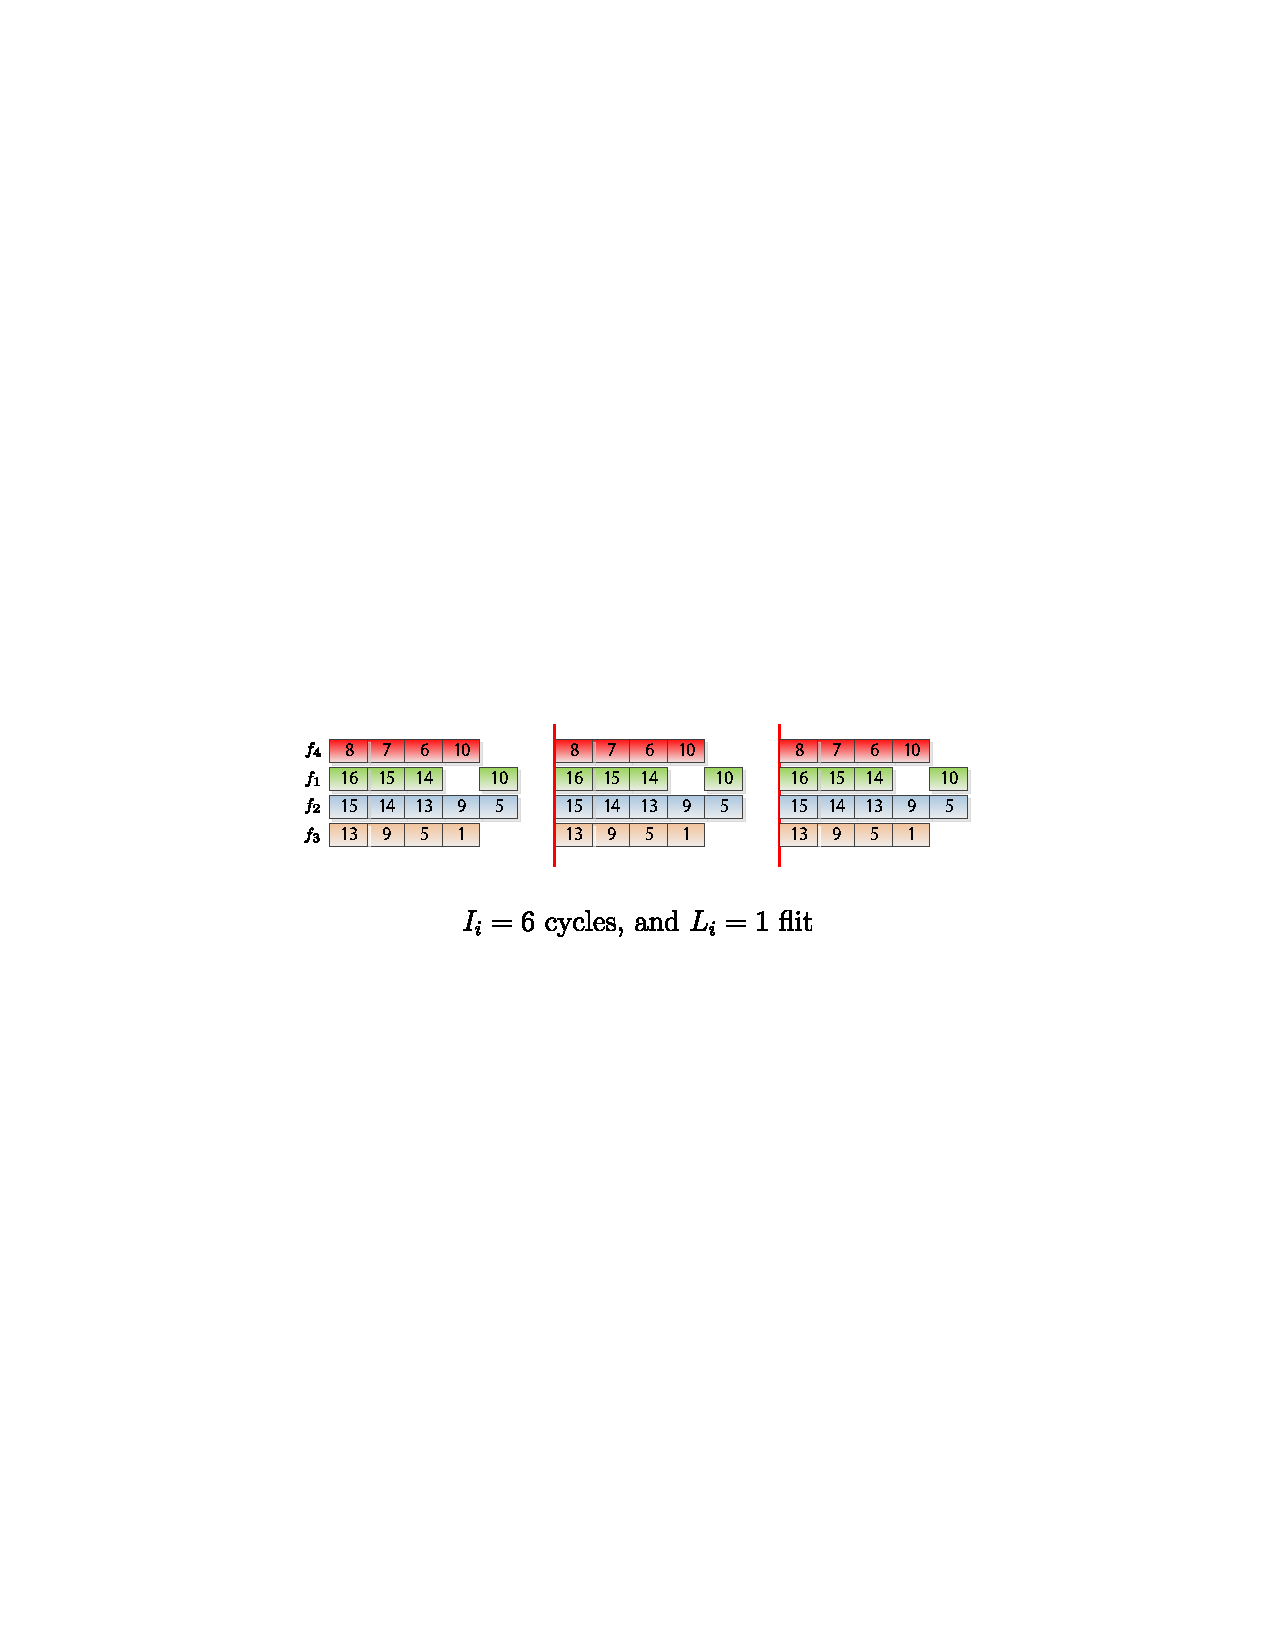
\includegraphics[scale=0.7]{figures/inaccurate.pdf}\\
  \caption{Time line graph of the four flows in Fig. \ref{topology}. Each block represents a router, and the color of the block means which flow are occupying the router at this time instance.}\label{inaccurate}
\end{figure}

\subsubsection{Buffer Optimization}
The proposed LLBA method \cite{189} can give the required buffer size of each VC to prevent flow control, this buffer size can be further reduced as long as the deadline is not violated. In this section, we try to demonstrate that, the RTC method can optimize the buffer size further by taking the flow control into consideration. Suppose the injection period $I_i=20$ and packet size $F_i=4$ ($i=1,2,3,4$), following the same configuration with the previous subsection, we can get the end-to-end latency for the four flows, which are 11, 12, 11 and 7, respectively. We can also get the buffer size reserved at each router with LLBA method, which are $(1,1,1,4)$, $(1,1,1,1,1)$, $(4,4,1,1)$ and $(1,1,1,1)$, respectively. We change the deadline constraint from 15 cycle to 27 cycle, and compute the required buffer size for each flow with our buffer optimization algorithm, the result is shown in Table \ref{LLBAvsRTC}.
\begin{table*}[htbp]
\centering
\caption{\label{LLBAvsRTC}buffer requirement comparison}
\begin{tabular}{|c|c|c|c|c|c|}
\hline
\multirow{2}{*}{Deadline}  & $f_1$  &   $f_2$   &   $f_3$   &   $f_4$   &   \multirow{2}{*}{Required Buffer Size} \\
($D_1$, $D_2$, $D_3$, $D_4$)    &   ($B_{16}$, $B_{15}$, $B_{14}$, $B_{10}$)  &   ($B_{15}$, $B_{14}$, $B_{13}$, $B_{9}$, $B_5$)  & ($B_{13}$, $B_{9}$, $B_{5}$, $B_{1}$)   &    ($B_{8}$, $B_{7}$, $B_{6}$, $B_{10}$)   &   \\
\hline
(15,15,15,15)   &   (1,1,1,2)   &   (2,1,1,1,1) &   (4,4,1,1)   &   (1,1,1,1)   &   25\\
\hline
(17,17,17,17)   &   (1,1,1,2)   &   (2,1,1,1,1) &   (3,3,1,1)   &   (1,1,1,1)   &   23\\
\hline
(19,19,19,19)   &   (1,1,1,2)   &   (2,1,1,1,1) &   (2,2,1,1)   &   (1,1,1,1)   &   22\\
\hline
(21,21,21,21)   &   (1,1,1,2)   &   (1,1,1,1,1) &   (2,2,1,1)   &   (1,1,1,1)   &   20\\
\hline
(23,23,23,23)   &   (1,1,1,1)   &   (1,1,1,1,1) &   (2,2,1,1)   &   (1,1,1,1)   &   19\\
\hline
(25,25,25,25)   &   (1,1,1,1)   &   (1,1,1,1,1) &   (2,2,1,1)   &   (1,1,1,1)   &   19\\
\hline
(27,27,27,27)   &   (1,1,1,1)   &   (1,1,1,1,1) &   (1,1,1,1)   &   (1,1,1,1)   &   17\\
\hline
\end{tabular}
\end{table*}

\subsection{Comparison with Network Calculus and Simulation}\label{dnccmp}
In this subsection, we present the numerical results to demonstrate the tightness and improvement of our method over DNC method proposed in \cite{Qian489900}. The correctness of our latency model and buffer optimization algorithm is verified by simulation. We modified the switch allocator of a modular open source NoC simulator, Heterogenous Networks-on-Chip (HNoCs) \cite{6404157}, to support fixed-priority scheduling, and collect the maximal end-to-end packet delay at each destination IP core. We can obtain the arrival curve according to the method introduced in subsection \ref{traffic}. In \cite{Qian489900}, the authors derived the service curve for each contention flow at the same input router. But, these service curves can only be used to derive the latency of injection router, for the service curve of each flow at subsequent router, the service curve should be computed with the same procedure as \cite{qian2009analysis}. We set the clock cycle as $T=2ns$, flit injection rate as $0.1$ flit/cycle, buffer depth as $B=4$ flits, credit feedback delay $\sigma=0$ cycle, and change the packet length from $1$ flit to $16$ flits. The priority of each flow in Fig. \ref{topology} is denoted as $P_i$ ($i=1,2,3,4$), and we assume $P_4=P_1>P_2>P_3$. The simulation results and numerical results of $f_3$ is plotted in Fig. \ref{comparison}. By comparison, we find that RTC can derive a much tighter latency bound compared with DNC, and the difference becomes larger when we increase the packet length.
\begin{figure}
  \centering
  % Requires \usepackage{graphicx}
  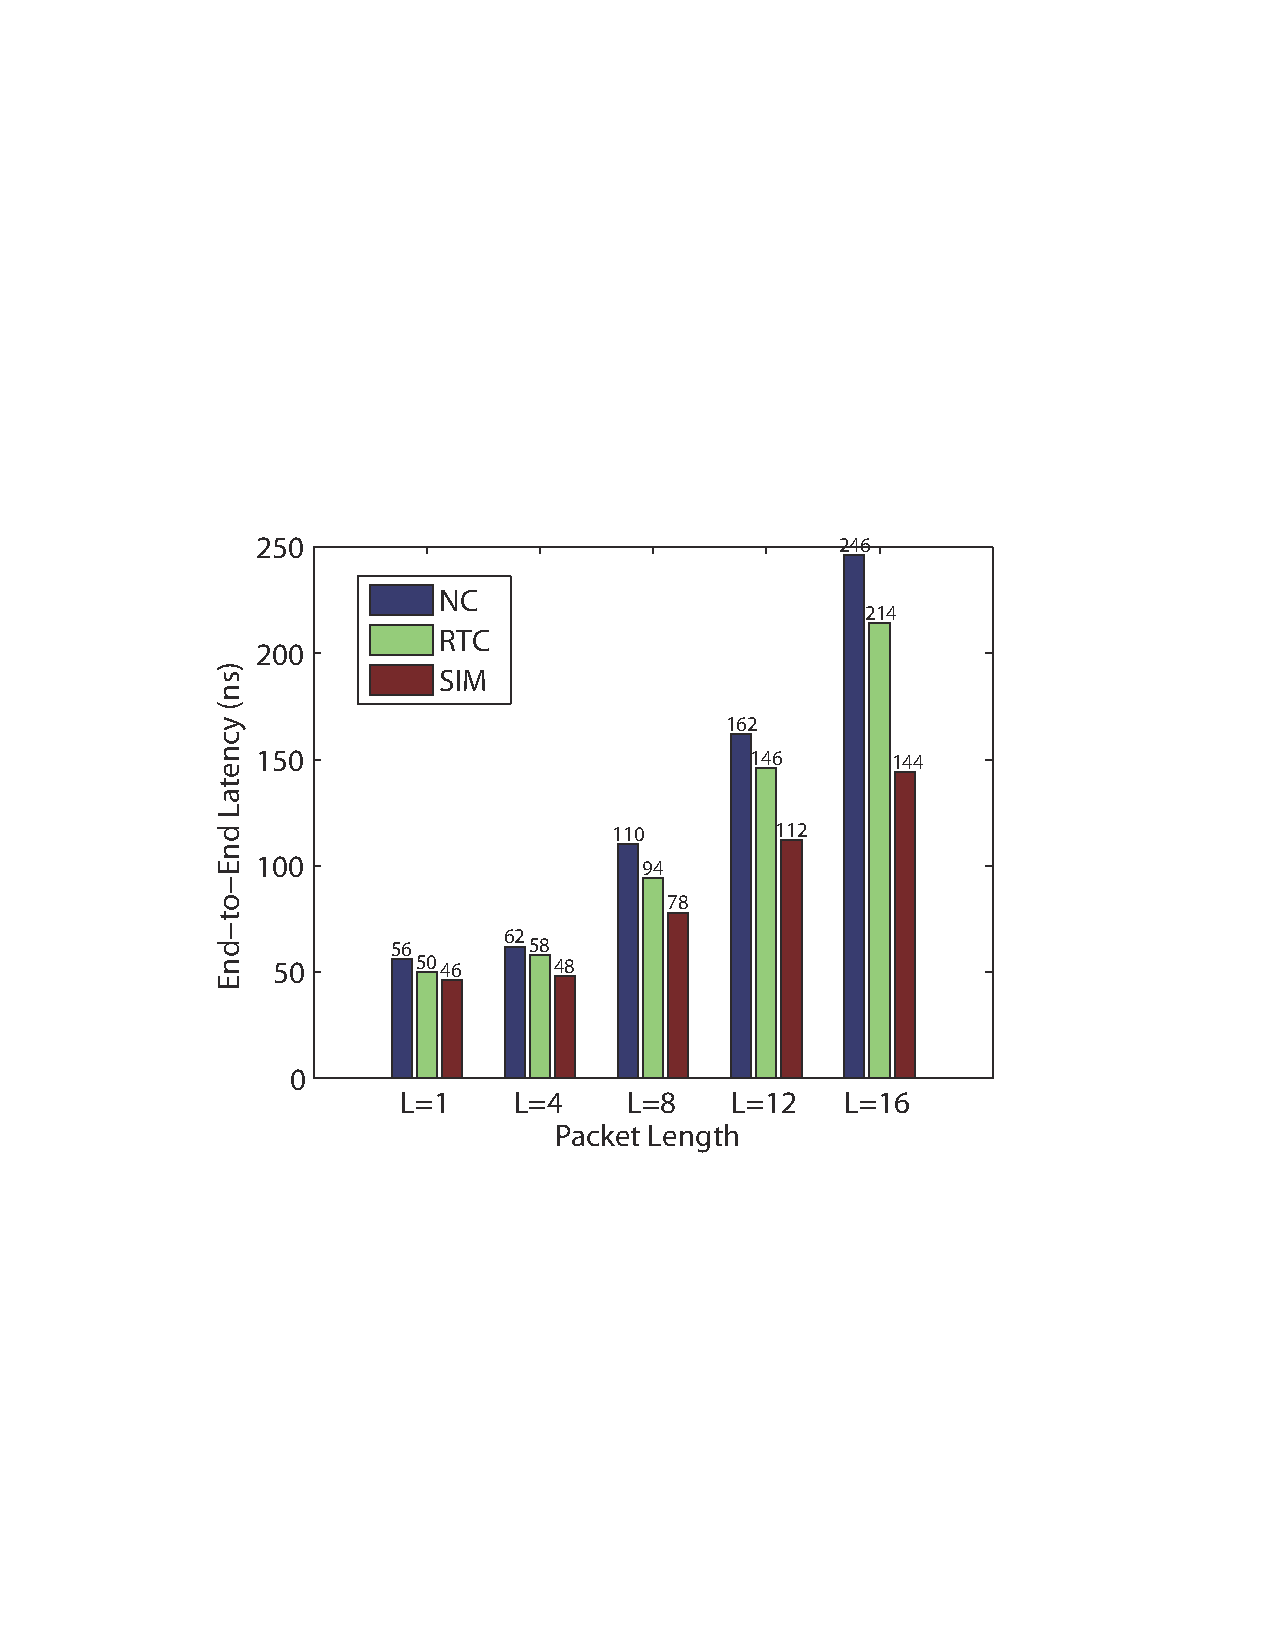
\includegraphics[scale=0.6]{figures/comparison.pdf}\\
  \caption{Comparison with network calculus and simulation}\label{comparison}
\end{figure}

Next, we explain the reason why our method outperform the DNC based method proposed in \cite{Qian489900}. As implied by Theorem 1.72 in \cite{Boudec2001Network}, the maximal service curve of current router can limit the arrival curve of next router, which leads to a tighter leftover service curve at next router for the other flows. To demonstrate this, let $B=4$ flits, $L=4$ flits, $\sigma=0$ cycle and $T=2ns$, we obtained the calculated service curve for flow $f_2$ both with DNC and RTC, as shown in Fig. \ref{loose}. The numerical calculation was carried out with RTC toolbox. From Fig. \ref{loose}, we find that, the calculated service curve with RTC is much 'better' than DNC, which explains why the RTC can produce better results.
\begin{figure}
  \centering
  % Requires \usepackage{graphicx}
  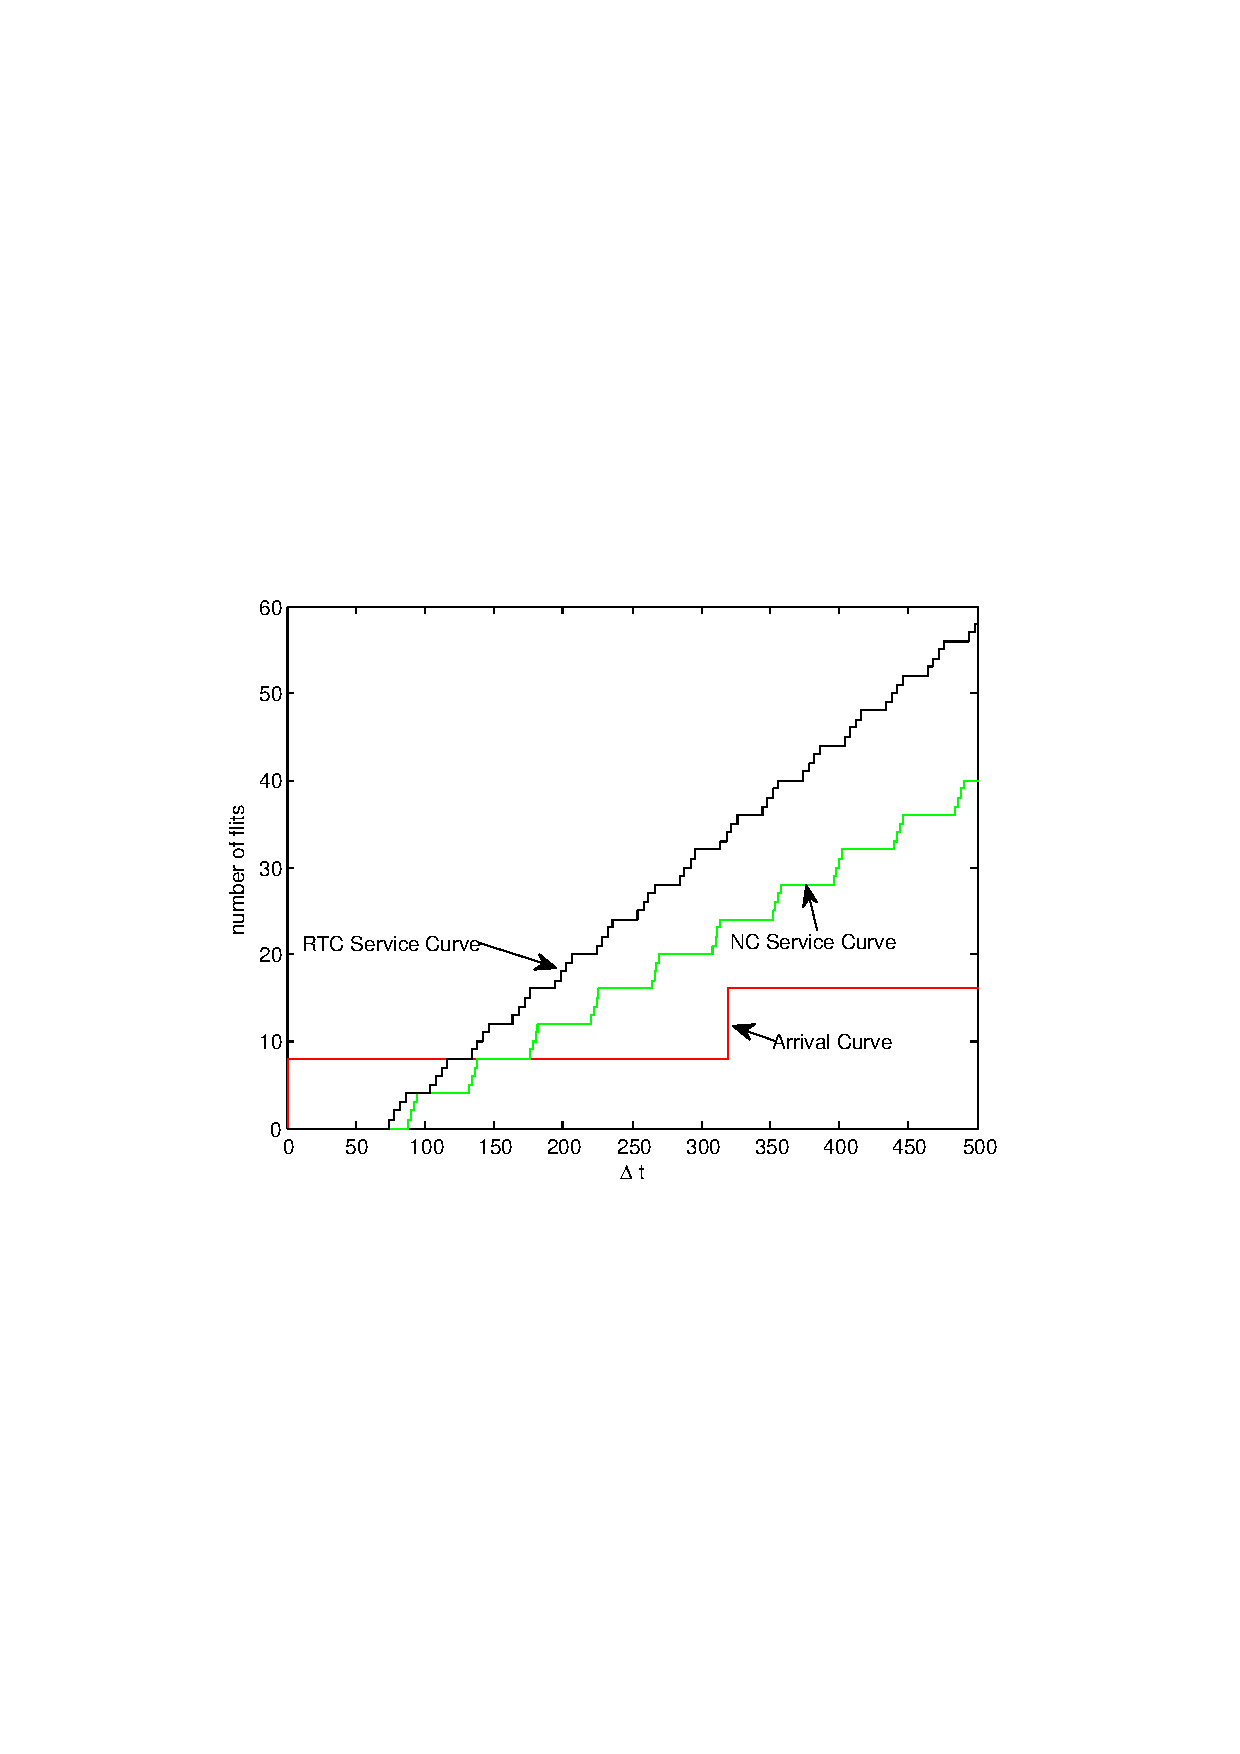
\includegraphics[scale=0.6]{figures/loose.pdf}\\
  \caption{Comparison of service curve computed with real-time calculus and network calculus}\label{loose}
\end{figure}

As has shown in previous subsections, the DNC based method \cite{Qian489900} can handle some circumstances that FLA and LLA can not be applied. This motivate us to optimize the buffer size of NoC with our method. Let the flit injection rate be $0.1$ flit/cycle, feedback delay $\sigma=0$ cycle, packet length $L=16$ flits and change the VC buffer depth from 4 flits to 10 flits, we compare the theoretical bound computed with DNC and our method, as shown in Fig. \ref{buffer}. It clear that, our method outperform the DNC based method, because it gives much tight bound for both $f_2$ and $f_3$. Further, if we set the deadline of $f_2$ and $f_3$ to 150ns, with our method, we can found that $B=8$ flits is sufficient enough to guarantee the delay bound. While the DNC based estimation is larger than $10$ flits. We also observed from Fig. \ref{buffer} that, the high priority flows (i.e. $f_1$ and $f_4$) are very insensitive to the buffer depths, which motivate us to allocate small buffers for these flows to reduce the area and power cost. We also observed that, for the priority-aware NoC, the lower priorities, the higher blocking ratios, thus leading to a larger buffer requirement.
\begin{figure*}
  \centering
  % Requires \usepackage{graphicx}
  \includegraphics[scale=0.5]{figures/buffer.pdf}\\
  \caption{End-to-end flows with different buffer size}\label{buffer}
\end{figure*}

\section{Conclusion}\label{conclusion}
The priority-aware wormhole-switched NoC is a promising platform for the on-chip real-time communication if the worst-case performance can be accurately analyzed and guaranteed. Simulation is not competent for this purpose because it is difficult to cover all the corner cases. In this paper, we propose an RTC based analytical model to achieve this goal. We first build the traffic model and service model for this NoC, and propose a novel method to derive the upper service curve of window flow control. Then, based on the proposed RTC model, we proposed an end-to-end latency analyzing algorithm and a buffer optimization algorithm. The latency analyzing algorithm can be implemented in RTC toolbox to compute the end-to-end latency for each flow automatically, to verify whether all these flows meet their deadline under this configuration. To improve the calculated delay bound, we proposed the concept of collapsible sub-path. The proposed buffer optimization algorithm can optimize the buffer size iteratively, from high-priority flows to low-priority flows. It can also be implemented with RTC toolbox to perform the buffer optimization automatically under the constraint of deadline. Experiment results demonstrate that, our method outperforms the conventional analytical methods, e.g. LLA and DNC, when the tightness of performance bound are considered. Our results can also be applied to the mapping, routing and power optimization of NoC.

\section*{Acknowledgement}
The authors would thank the reviewers for their suggestions and comments, and all the experiments are carried out at Integrated Microsystem Lab (IML) of McGill University. This research is supported by High Technology Research and Development Program of China (Grant No. 2012AA012201, 2012AA011902).

\bibliographystyle{unsrt}
\bibliography{Docear}

\end{document} 